% =============================================================
% 6 Анализ радиального подшипника шарошечного долота
% =============================================================
\chapter{Анализ рельефного радиального подшипника шарошечного долота}

\section{Объект исследования и исходные данные}

Объектом исследования в настоящей главе является радиальный
подшипник скольжения опоры шарошки трёхшарошечного долота~\cite{bashmur2024a,bashmur2024b}.
Цапфа (лапа долота) неподвижна относительно корпуса; шарошка
вращается вокруг цапфы. Подшипниковый узел воспринимает
радиальные нагрузки от долота и обеспечивает смазку при тяжёлых
условиях эксплуатации: высокие нагрузки, низкая скорость
скольжения, ограниченная подача смазки.

В отличие от подшипника насоса (глава~5), опора шарошечного долота
работает при скорости скольжения~$U_{\mathrm{eq}}$, примерно
в~90 раз меньшей, и нагрузке $F_{\mathrm{ext}} = 6\,000$~Н на цапфу. Вследствие малой
скорости гидродинамическое давление невелико, и подшипник
функционирует в смешанном или граничном режиме смазки. Применение
детерминированных микроструктур рабочей поверхности направлено
на повышение гидродинамической составляющей несущей способности
и улучшение условий смазки~\cite{bashmur2022,bashmur2023a,bashmur2023b,guo2005}.

Кинематика узла определяется вращением шарошки. Угловая скорость
вращения долота (корпуса):
\begin{equation}
  \omega = \frac{2\pi n}{60},
  \label{eq:bit_omega}
\end{equation}
где $n$~-- частота вращения долота, об/мин. Относительная угловая
скорость шарошки относительно цапфы:
\begin{equation}
  \omega_{\mathrm{rel}} = \omega
    \left(\frac{R_b}{R_k} - 1\right),
  \label{eq:bit_omega_rel}
\end{equation}
где $R_b$~-- радиус долота, $R_k$~-- радиус шарошки.
Эквивалентная скорость скольжения на поверхности цапфы:
\begin{equation}
  U_{\mathrm{eq}} = |\omega_{\mathrm{rel}}|\, R,
  \label{eq:bit_Ueq}
\end{equation}
где $R$~-- радиус цапфы. Подстановка числовых значений даёт
$U_{\mathrm{eq}} \approx 0{,}124$~м/с.

Нагрузка на цапфу определяется из осевой нагрузки на долото~$F_a$.
Нагрузка на одну шарошку при равномерном распределении:
\begin{equation}
  F_{\mathrm{cone}} = \frac{F_a}{3}.
  \label{eq:bit_Fcone}
\end{equation}
В расчётах принято $F_a = 150$~кН, что соответствует
$F_{\mathrm{cone}} = 50$~кН.
Радиальная нагрузка на цапфу:
\begin{equation}
  F_{\mathrm{ext}} = k_L \cdot F_{\mathrm{cone}},
  \label{eq:bit_Fext}
\end{equation}
где $k_L = 0{,}12$~-- коэффициент передачи нагрузки на цапфу
(инженерное оценочное допущение; далее принято $k_L = 0{,}12$).

Основные параметры подшипника сведены в таблицу~\ref{tab:bit_params}.

\begin{table}[!ht]
\centering
\caption{Параметры радиального подшипника скольжения опоры шарошки}
\label{tab:bit_params}
\begin{tabularx}{\textwidth}{|X|c|c|c|}
\hline
\multicolumn{1}{|c|}{\textbf{Параметр}} & \textbf{Обозначение} & \textbf{Значение} & \textbf{Единица} \\
\hline
Радиус цапфы              & $R$              & 30{,}0  & мм \\
\hline
Длина подшипника          & $L$              & 40{,}0  & мм \\
\hline
Радиальный зазор          & $c$              & 60      & мкм \\
\hline
Относительный зазор       & $\psi = c/R$     & $2{,}00 \times 10^{-3}$ & -- \\
\hline
Отношение $L/D$           & $L/D$            & 0{,}667 & -- \\
\hline
Радиус долота             & $R_b$            & 107{,}5 & мм \\
\hline
Радиус шарошки            & $R_k$            & 72{,}0  & мм \\
\hline
Частота вращения          & $n$              & 80      & об/мин \\
\hline
Угловая скорость          & $\omega$         & 8{,}38  & рад/с \\
\hline
Эквивалентная скорость    & $U_{\mathrm{eq}}$ & 0{,}124 & м/с \\
\hline
Динамическая вязкость     & $\mu_0$          & $5{,}5 \times 10^{-2}$ & Па$\cdot$с \\
\hline
Температура               & $T_0$            & 80      & $^{\circ}$C \\
\hline
Суммарная шероховатость   & $\sigma_{\mathrm{eq}}$ & 0{,}89 & мкм \\
\hline
Коэффициент передачи      & $k_L$            & 0{,}12  & -- \\
\hline
Нагрузка на цапфу         & $F_{\mathrm{ext}}$ & 6\,000 & Н \\
\hline
Давление кавитации        & $p_{\mathrm{cav}}$ & 0     & Па \\
\hline
\end{tabularx}
\end{table}

\FloatBarrier

Схема опоры шарошки представлена на рисунке~\ref{fig:bit_scheme}.

\begin{figure}[!ht]
\centering
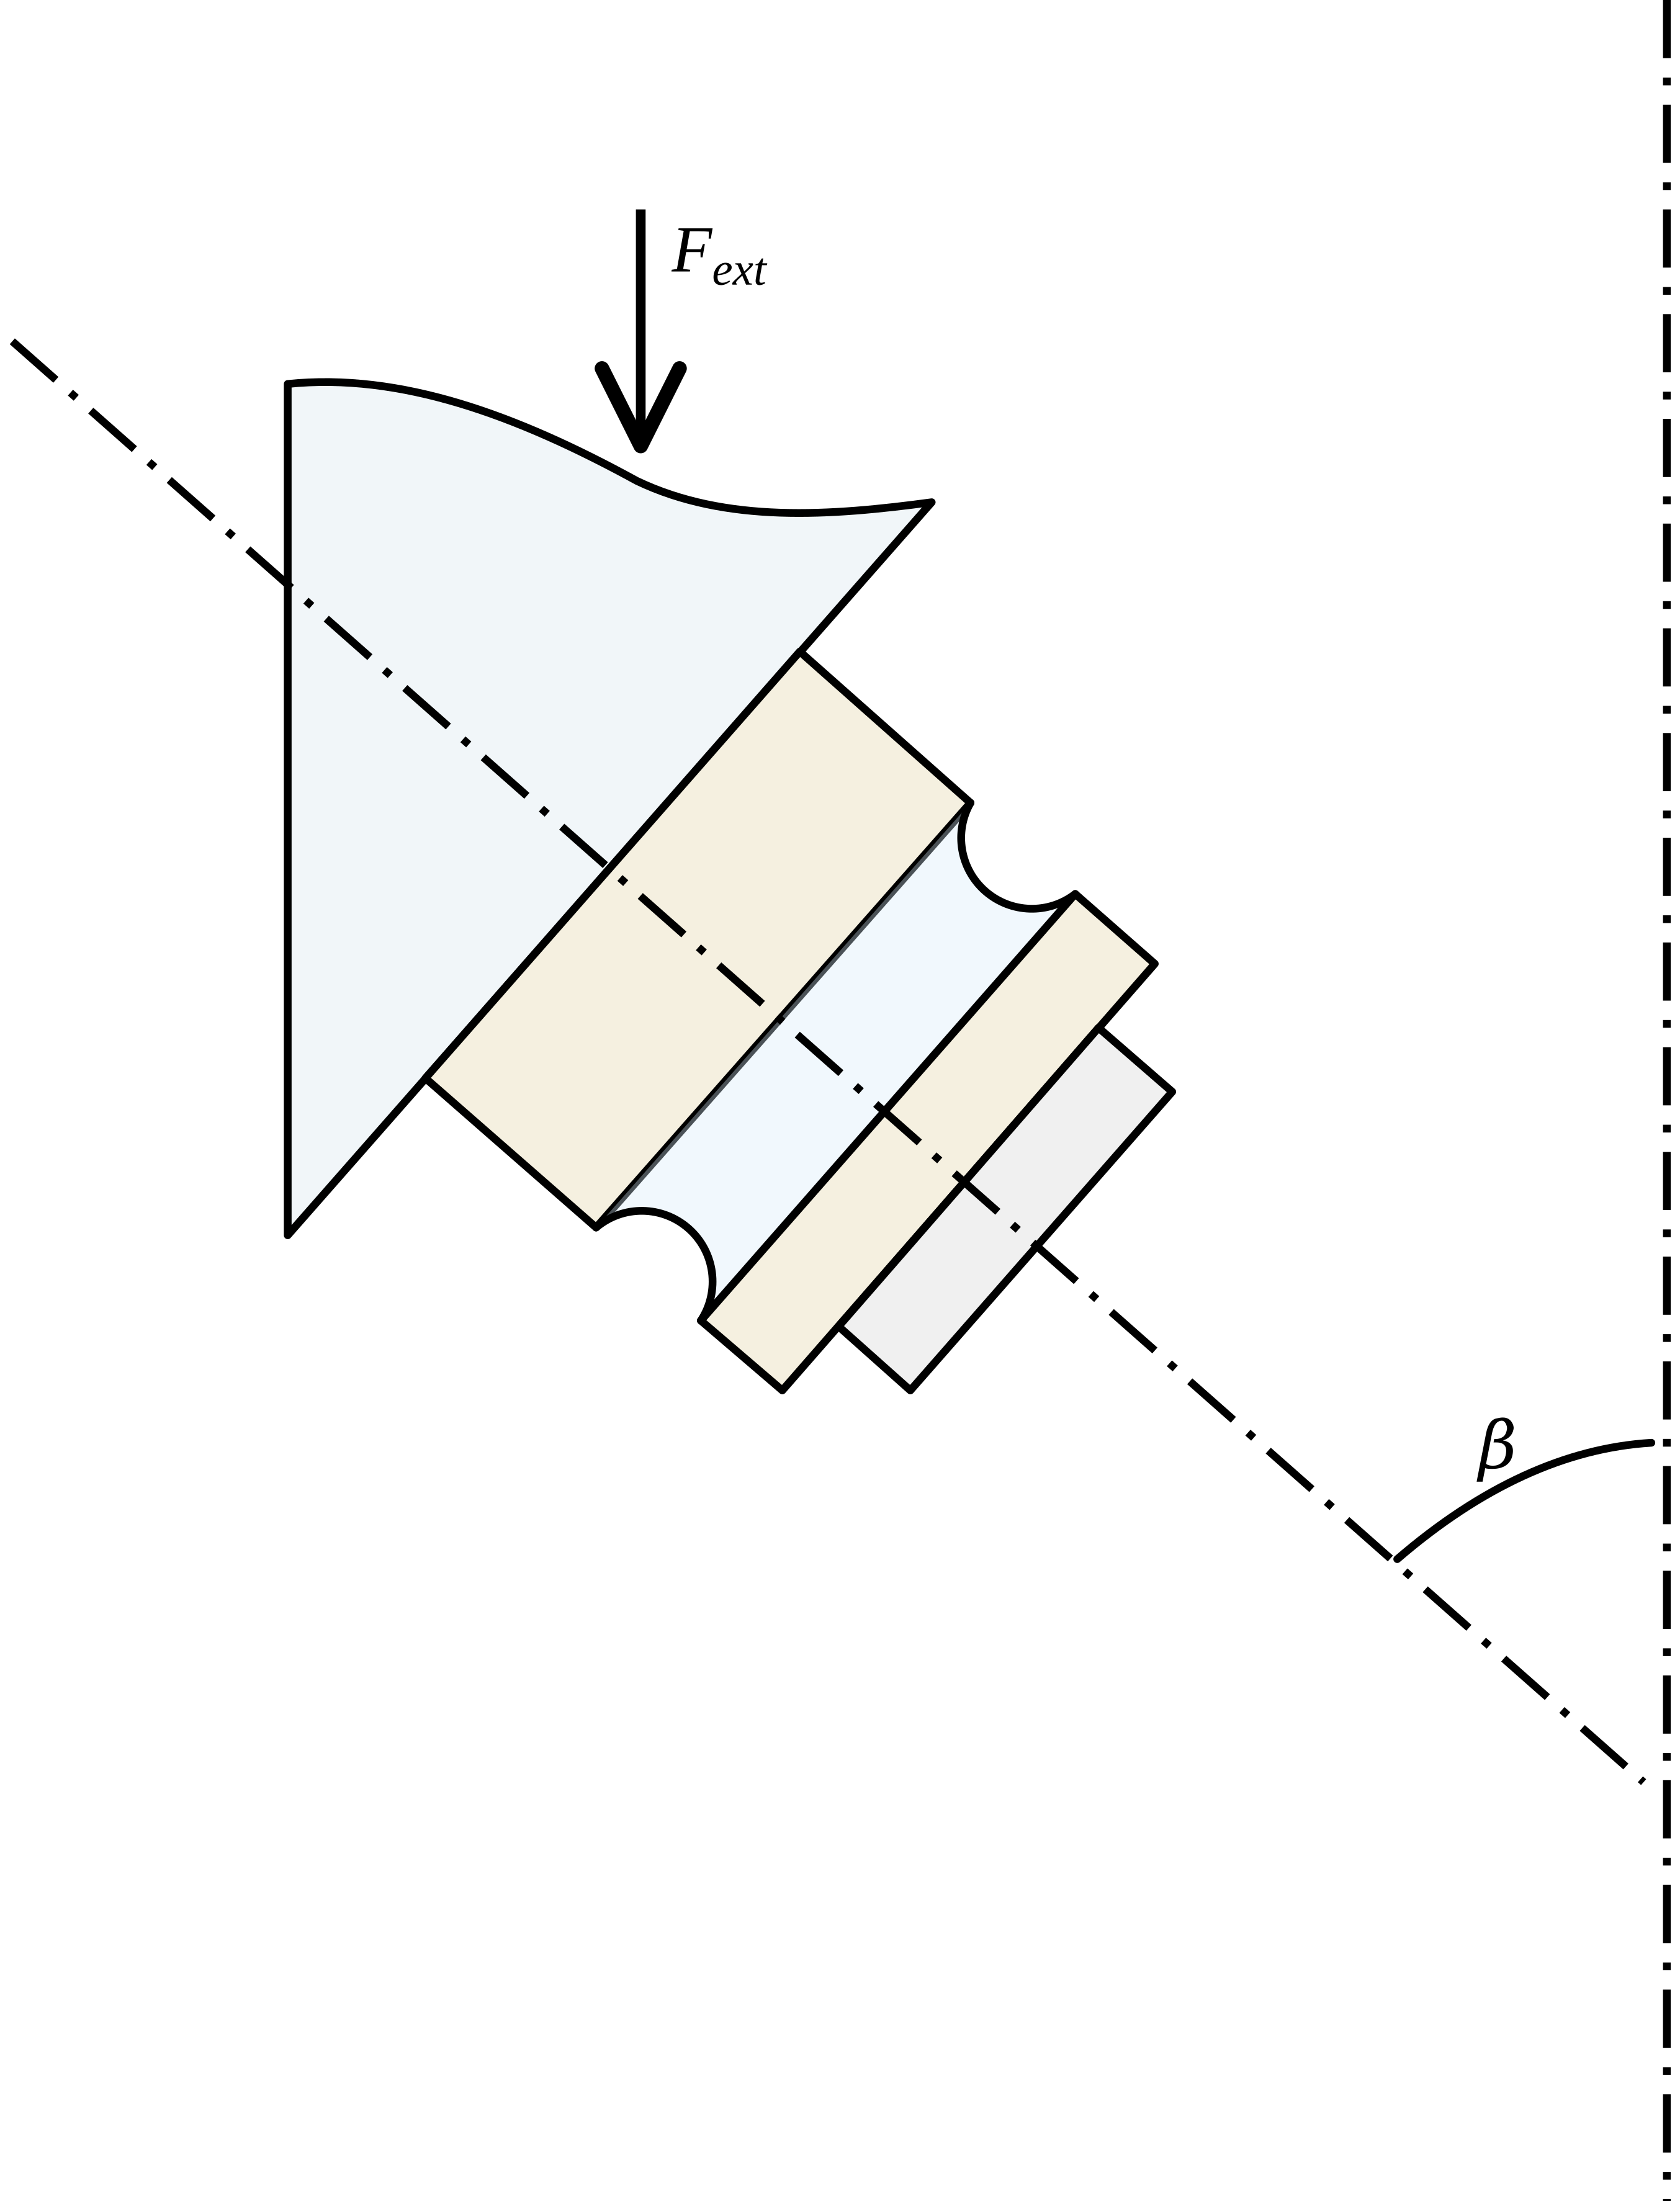
\includegraphics[width=\textwidth,height=0.9\textheight,keepaspectratio]{figures/ch06/fig_6_1.png}
\caption{Схема опоры шарошки трёхшарошечного долота}
\label{fig:bit_scheme}
\end{figure}

\FloatBarrier


\section{Постановка задачи}\label{sec:problem_statement_ch6}

Расчётная область представляет собой развёрнутую поверхность
смазочного зазора $(\theta, z) \in [0,\,2\pi] \times [-L/2,\,L/2]$,
где $\theta$~-- окружная координата, $z$~-- осевая координата.
В тексте главы окружная координата обозначается~$\theta$;
на рисунках ось подписана~$\varphi$; везде $\theta \equiv \varphi$.
При переходе к безразмерным переменным (подраздел~2.1.6)
осевая координата нормируется на полудлину: $Z = 2z/L$,
так что $Z \in [-1,\,1]$.

Для гладкого цилиндрического подшипника безразмерная толщина
зазора определяется законом~\eqref{eq:journal_h_ch5}:
\begin{equation}
  H(\theta) = 1 + \varepsilon\cos\theta,
  \label{eq:bit_h}
\end{equation}
где $\varepsilon = e/c$~-- относительный эксцентриситет
($0 \leq \varepsilon < 1$). Для подшипника с детерминированными
микроструктурами толщина зазора записывается в виде
суперпозиции~\eqref{eq:journal_h_tex_ch5}:
\begin{equation}
  H = H_0(\theta) + \Delta H_t(\theta, Z).
  \label{eq:bit_h_tex}
\end{equation}
где $H_0(\theta) = 1 + \varepsilon\cos\theta$~-- базовый зазор гладкого подшипника~\eqref{eq:bit_h}, $\Delta H_t$~-- добавка микрорельефа (подраздел~2.2).

Распределение давления описывается безразмерным уравнением
Рейнольдса~\eqref{eq:reynolds_nondim} с параметром
анизотропии~$\Lambda$~\eqref{eq:nondim_Lambda}.

Граничные условия: по окружной координате~$\theta$ поле давления
периодично ($P(\theta = 0) = P(\theta = 2\pi)$); на торцах
подшипника давление равно атмосферному ($P = 0$ при $Z = \pm 1$).
Кавитация учитывается по условию Рейнольдса: $P \geq 0$.

В отличие от главы~5, где эксцентриситет задавался как входной
параметр и вычислялась несущая сила~$F(\varepsilon)$, в настоящей
главе рассматривается обратная задача: задаётся внешняя нагрузка
$F_{\mathrm{ext}}$, а равновесный эксцентриситет~$\varepsilon^*$
определяется из условия равновесия:
\begin{equation}
  F(\varepsilon^*) = F_{\mathrm{ext}}.
  \label{eq:bit_equilibrium}
\end{equation}
Решение уравнения~\eqref{eq:bit_equilibrium} выполняется методом
бисекции по~$\varepsilon \in [0{,}05;\; 0{,}97]$ с допуском~$1\,\%$.

Для оценки режима смазки вводится минимальная толщина плёнки:
\begin{equation}
  h_{\min} = c\,(1 - \varepsilon),
  \label{eq:bit_hmin}
\end{equation}
а также параметр плёнки:
\begin{equation}
  \lambda = \frac{h_{\min}}{\sigma_{\mathrm{eq}}},
  \label{eq:bit_lambda}
\end{equation}
где $\sigma_{\mathrm{eq}}$~-- суммарная шероховатость поверхностей.
Классификация режимов смазки по параметру~$\lambda$:
$\lambda < 1$~-- граничный режим;
$1 \leq \lambda \leq 3$~-- смешанный режим;
$\lambda > 3$~-- гидродинамический режим.

Для сравнительной оценки условий работы узла вводится
$PV$-параметр:
\begin{equation}
  p_0 = \frac{F}{2\,R\,L}, \qquad
  PV = p_0 \cdot U_{\mathrm{eq}},
  \label{eq:bit_PV}
\end{equation}
и индекс износа:
\begin{equation}
  I_w = \frac{PV}{h_{\min}}.
  \label{eq:bit_Iw}
\end{equation}
Величина~$I_w$ является суррогатным сравнительным
индексом, характеризующим интенсивность изнашивания; строгое
соответствие закону Арчарда не предполагается.

Допущения, принятые в настоящей главе, включают: изотермическое
приближение ($T = T_0$, $\mu = \mathrm{const}$), постоянство
плотности ($\rho = \mathrm{const}$) и кавитация по условию
Рейнольдса ($P \geq 0$).


\section{Результаты для гладкого подшипника}

При расчётном пределе эксцентриситета $\varepsilon = 0{,}97$
гладкий подшипник развивает несущую силу
$F(\varepsilon = 0{,}97) = 1907$~Н. Это составляет около~$3{,}8\,\%$
от нагрузки на шарошку $F_{\mathrm{cone}} = F_a / 3 = 50\,000$~Н
и менее трети рабочей нагрузки $F_{\mathrm{ext}} = 6\,000$~Н.

Низкая несущая способность обусловлена малой скоростью скольжения
$U_{\mathrm{eq}} \approx 0{,}124$~м/с, примерно в~90 раз меньшей,
чем у подшипника насоса главы~5. Гидродинамическое давление
пропорционально скорости ($p \sim \mu_0\, U_{\mathrm{eq}}\, R / c^2$), поэтому даже
при предельном эксцентриситете несущая сила не достигает
$F_{\mathrm{ext}}$.

При рабочей нагрузке $F_{\mathrm{ext}} = 6\,000$~Н гладкий
подшипник не имеет равновесной рабочей точки в чисто
гидродинамической постановке. Режим смазки~-- смешанный или
граничный. Применение детерминированных микроструктур
рассматривается как средство повышения гидродинамической
составляющей несущей способности.


\section{Выбор и параметры микроструктуры}

В качестве элементов микрорельефа выбраны эллипсоидальные лунки
с профилем~\eqref{eq:profile_ellipsoidal}, расположенные
по шахматной схеме~\eqref{eq:layout_staggered}. Выбор типа
элемента и раскладки аналогичен главе~5 (подраздел~2.2).

Зона нанесения микроструктур определяется расположением области
максимального давления. В радиальном подшипнике максимум давления
формируется вблизи $\theta \approx \pi$ (зона минимального зазора).
Конфигурации~T1 и~T2 нанесены в секторе
$90^{\circ}$--$270^{\circ}$, включающем эту зону. Конфигурация~T3
нанесена в секторе $0^{\circ}$--$180^{\circ}$ (зона сходящегося
клина).

Параметры микроструктур (безразмерные полуоси~$A^*$, $B^*$)
пересчитаны под геометрию опоры шарошки ($R = 30$~мм,
$L = 40$~мм); числовые значения отличаются от конфигураций
главы~5 ($R = 35$~мм, $L = 56$~мм). Поэтому сравнение текстур
выполняется только внутри настоящей главы; прямое количественное
сопоставление с главой~5 не проводится.

Параметры рассматриваемых конфигураций приведены в
таблице~\ref{tab:bit_texture_configs}.

\begin{table}[!ht]
\centering
\caption{Параметры конфигураций текстуры для подшипника шарошечного долота}
\label{tab:bit_texture_configs}
\begin{tabularx}{\textwidth}{|X|c|c|c|c|}
\hline
\multicolumn{1}{|c|}{\textbf{Конфигурация}} & $\boldsymbol{H_p}$ & $\boldsymbol{A^*}$ & $\boldsymbol{B^*}$ & \textbf{Зона нанесения} \\
\hline
T1 & 0{,}20 & 0{,}0600 & 0{,}0367 & $90^{\circ}$--$270^{\circ}$ \\
\hline
T2 & 0{,}40 & 0{,}0600 & 0{,}0367 & $90^{\circ}$--$270^{\circ}$ \\
\hline
T3 & 0{,}20 & 0{,}0600 & 0{,}0367 & $0^{\circ}$--$180^{\circ}$ \\
\hline
\end{tabularx}
\end{table}


\section{Сравнение гладкого и текстурированного подшипников}

\textit{Рабочие точки при заданной нагрузке на цапфу.}
Все три конфигурации текстуры (T1--T3) обеспечивают равновесную
рабочую точку при $F_{\mathrm{ext}} = 6\,000$~Н; гладкий
подшипник рабочей точки не имеет. Результаты расчёта рабочих точек
сведены в таблицу~\ref{tab:bit_results}.

\begin{table}[!ht]
\centering
\caption{Характеристики подшипника в рабочей точке
  при $F_{\mathrm{ext}} = 6\,000$~Н}
\label{tab:bit_results}
\resizebox{\textwidth}{!}{%
\begin{tabular}{|l|c|c|c|c|c|c|c|c|}
\hline
\multicolumn{1}{|c|}{\textbf{Вар.}}
  & $\boldsymbol{\varepsilon}$
  & $\boldsymbol{F}$, Н
  & $\boldsymbol{\varphi}$, $^{\circ}$
  & $\boldsymbol{\mu_f}$
  & $\boldsymbol{h_{\min}}$, мкм
  & $\boldsymbol{\lambda}$
  & $\boldsymbol{PV}$, Па$\cdot$м/с
  & $\boldsymbol{I_w}$ \\
\hline
T1 & 0{,}966 & 6004 & 175{,}4 & 0{,}00123 & 2{,}04 & 2{,}28
   & 309\,981 & $1{,}5 \cdot 10^{11}$ \\
\hline
T2 & 0{,}956 & 6044 & 175{,}9 & 0{,}00107 & 2{,}66 & 2{,}98
   & 312\,090 & $1{,}2 \cdot 10^{11}$ \\
\hline
T3 & 0{,}969 & 5956 & 173{,}8 & 0{,}00136 & 1{,}85 & 2{,}07
   & 307\,503 & $1{,}7 \cdot 10^{11}$ \\
\hline
\end{tabular}%
}
\end{table}

\FloatBarrier

Все три конфигурации работают в смешанном режиме смазки
($1 \leq \lambda \leq 3$).

Приведённый коэффициент трения~$\mu_f$ соответствует
гидродинамической составляющей модели. В смешанном режиме
($\lambda < 3$) реальное трение в узле выше вследствие
дополнительного вклада контактного взаимодействия шероховатостей
поверхностей.

Конфигурация~T2 демонстрирует наилучшие характеристики:
наименьший эксцентриситет $\varepsilon = 0{,}956$, наибольший
минимальный зазор $h_{\min} = 2{,}66$~мкм, параметр плёнки
$\lambda = 2{,}98$~-- значение, наиболее близкое к границе
гидродинамического режима. Конфигурация~T3, в которой текстура
расположена вне зоны максимального давления, показывает наихудшие
значения~$h_{\min}$ и~$\lambda$.


\textit{Грузоподъёмность при расчётном пределе эксцентриситета.}
При расчётном пределе $\varepsilon = 0{,}97$ несущая сила
составляет: гладкий подшипник~-- $1\,907$~Н; T1~-- $7\,237$~Н;
T2~-- $7\,549$~Н; T3~-- $6\,212$~Н. Максимальная грузоподъёмность
конфигурации~T2 в~$3{,}96$ раза превышает значение гладкого
подшипника. Горизонталь $F_{\mathrm{ext}} = 6\,000$~Н пересекает
кривые~T1, T2, T3, но не кривую гладкого подшипника: рабочая точка
при заданной нагрузке существует только при наличии текстуры.

Зависимости несущей силы~$F(\varepsilon)$ для всех вариантов
представлены на рисунке~\ref{fig:bit_operating_points}.

\begin{figure}[!ht]
\centering
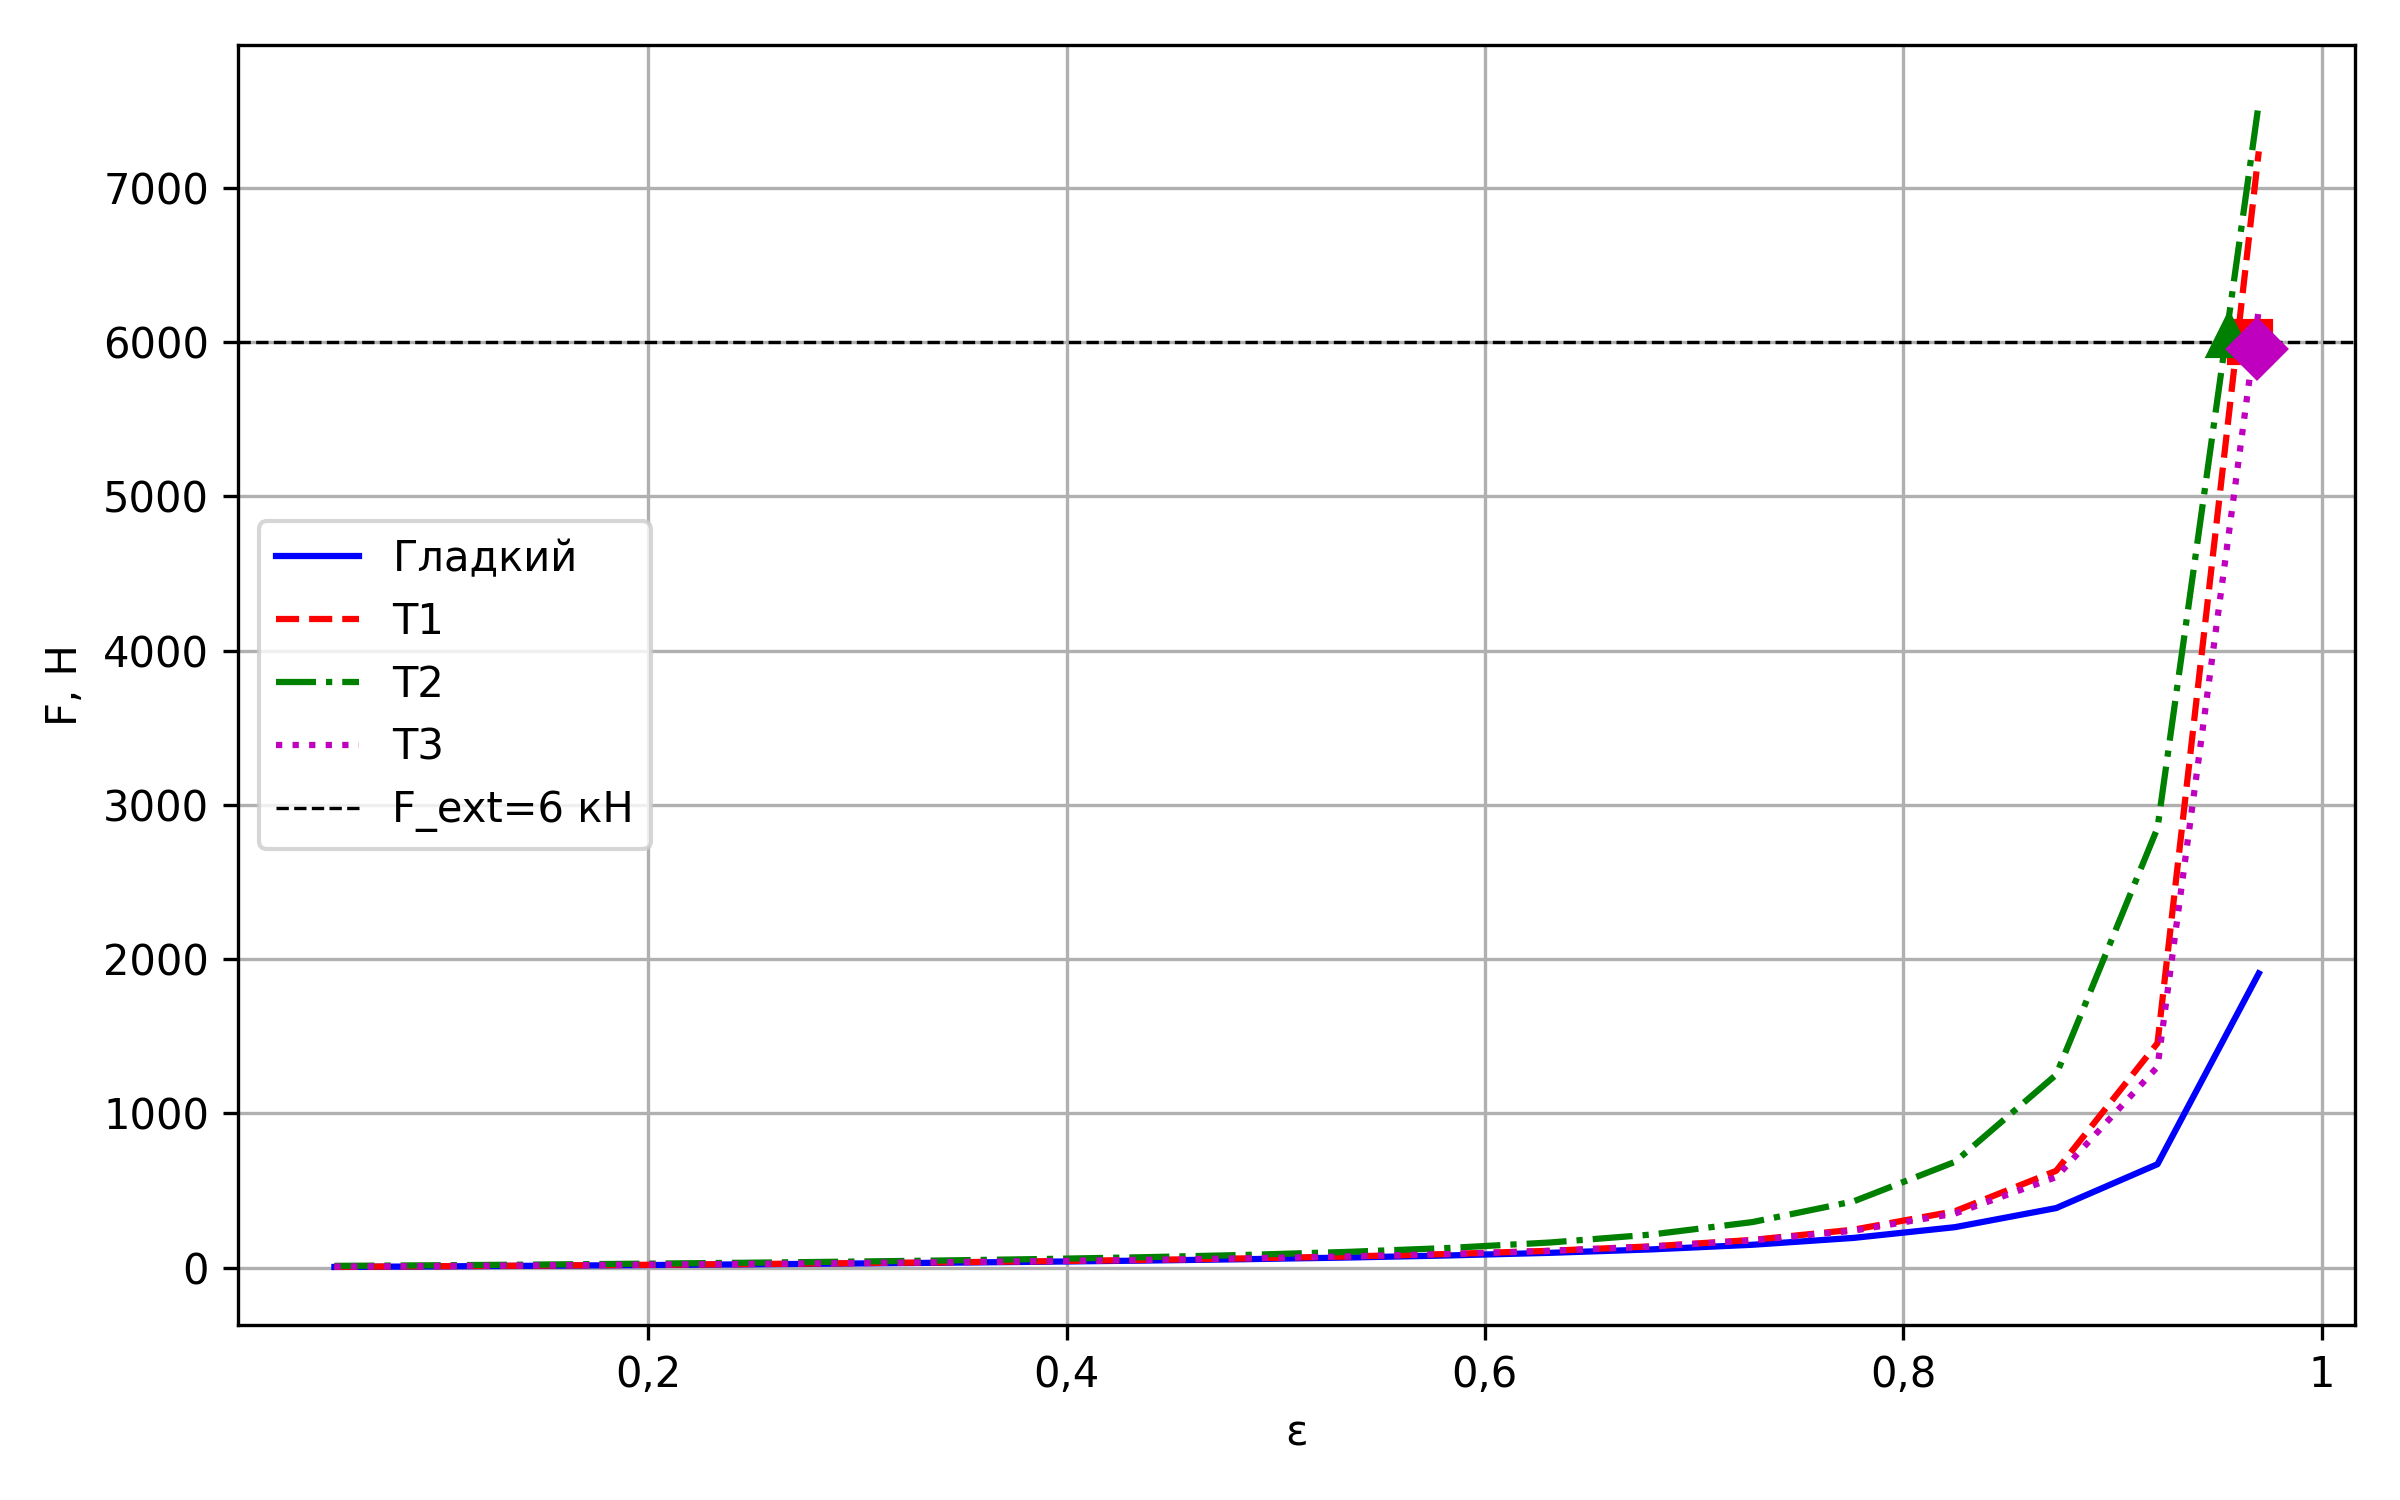
\includegraphics[width=\textwidth,height=0.9\textheight,keepaspectratio]{figures/ch06/fig_6_2.png}
\caption{Зависимость несущей силы $F$ от эксцентриситета $\varepsilon$
  для гладкого подшипника и конфигураций T1, T2, T3.
  Пунктирная горизонталь~-- рабочая нагрузка $F_{\mathrm{ext}} = 6\,000$~Н;
  маркеры~-- равновесные рабочие точки текстурированных конфигураций.}
\label{fig:bit_operating_points}
\end{figure}

\FloatBarrier

Параметр плёнки~$\lambda$ в рабочих точках текстурированных
конфигураций представлен на рисунке~\ref{fig:bit_lambda_comparison}.

\begin{figure}[!ht]
\centering
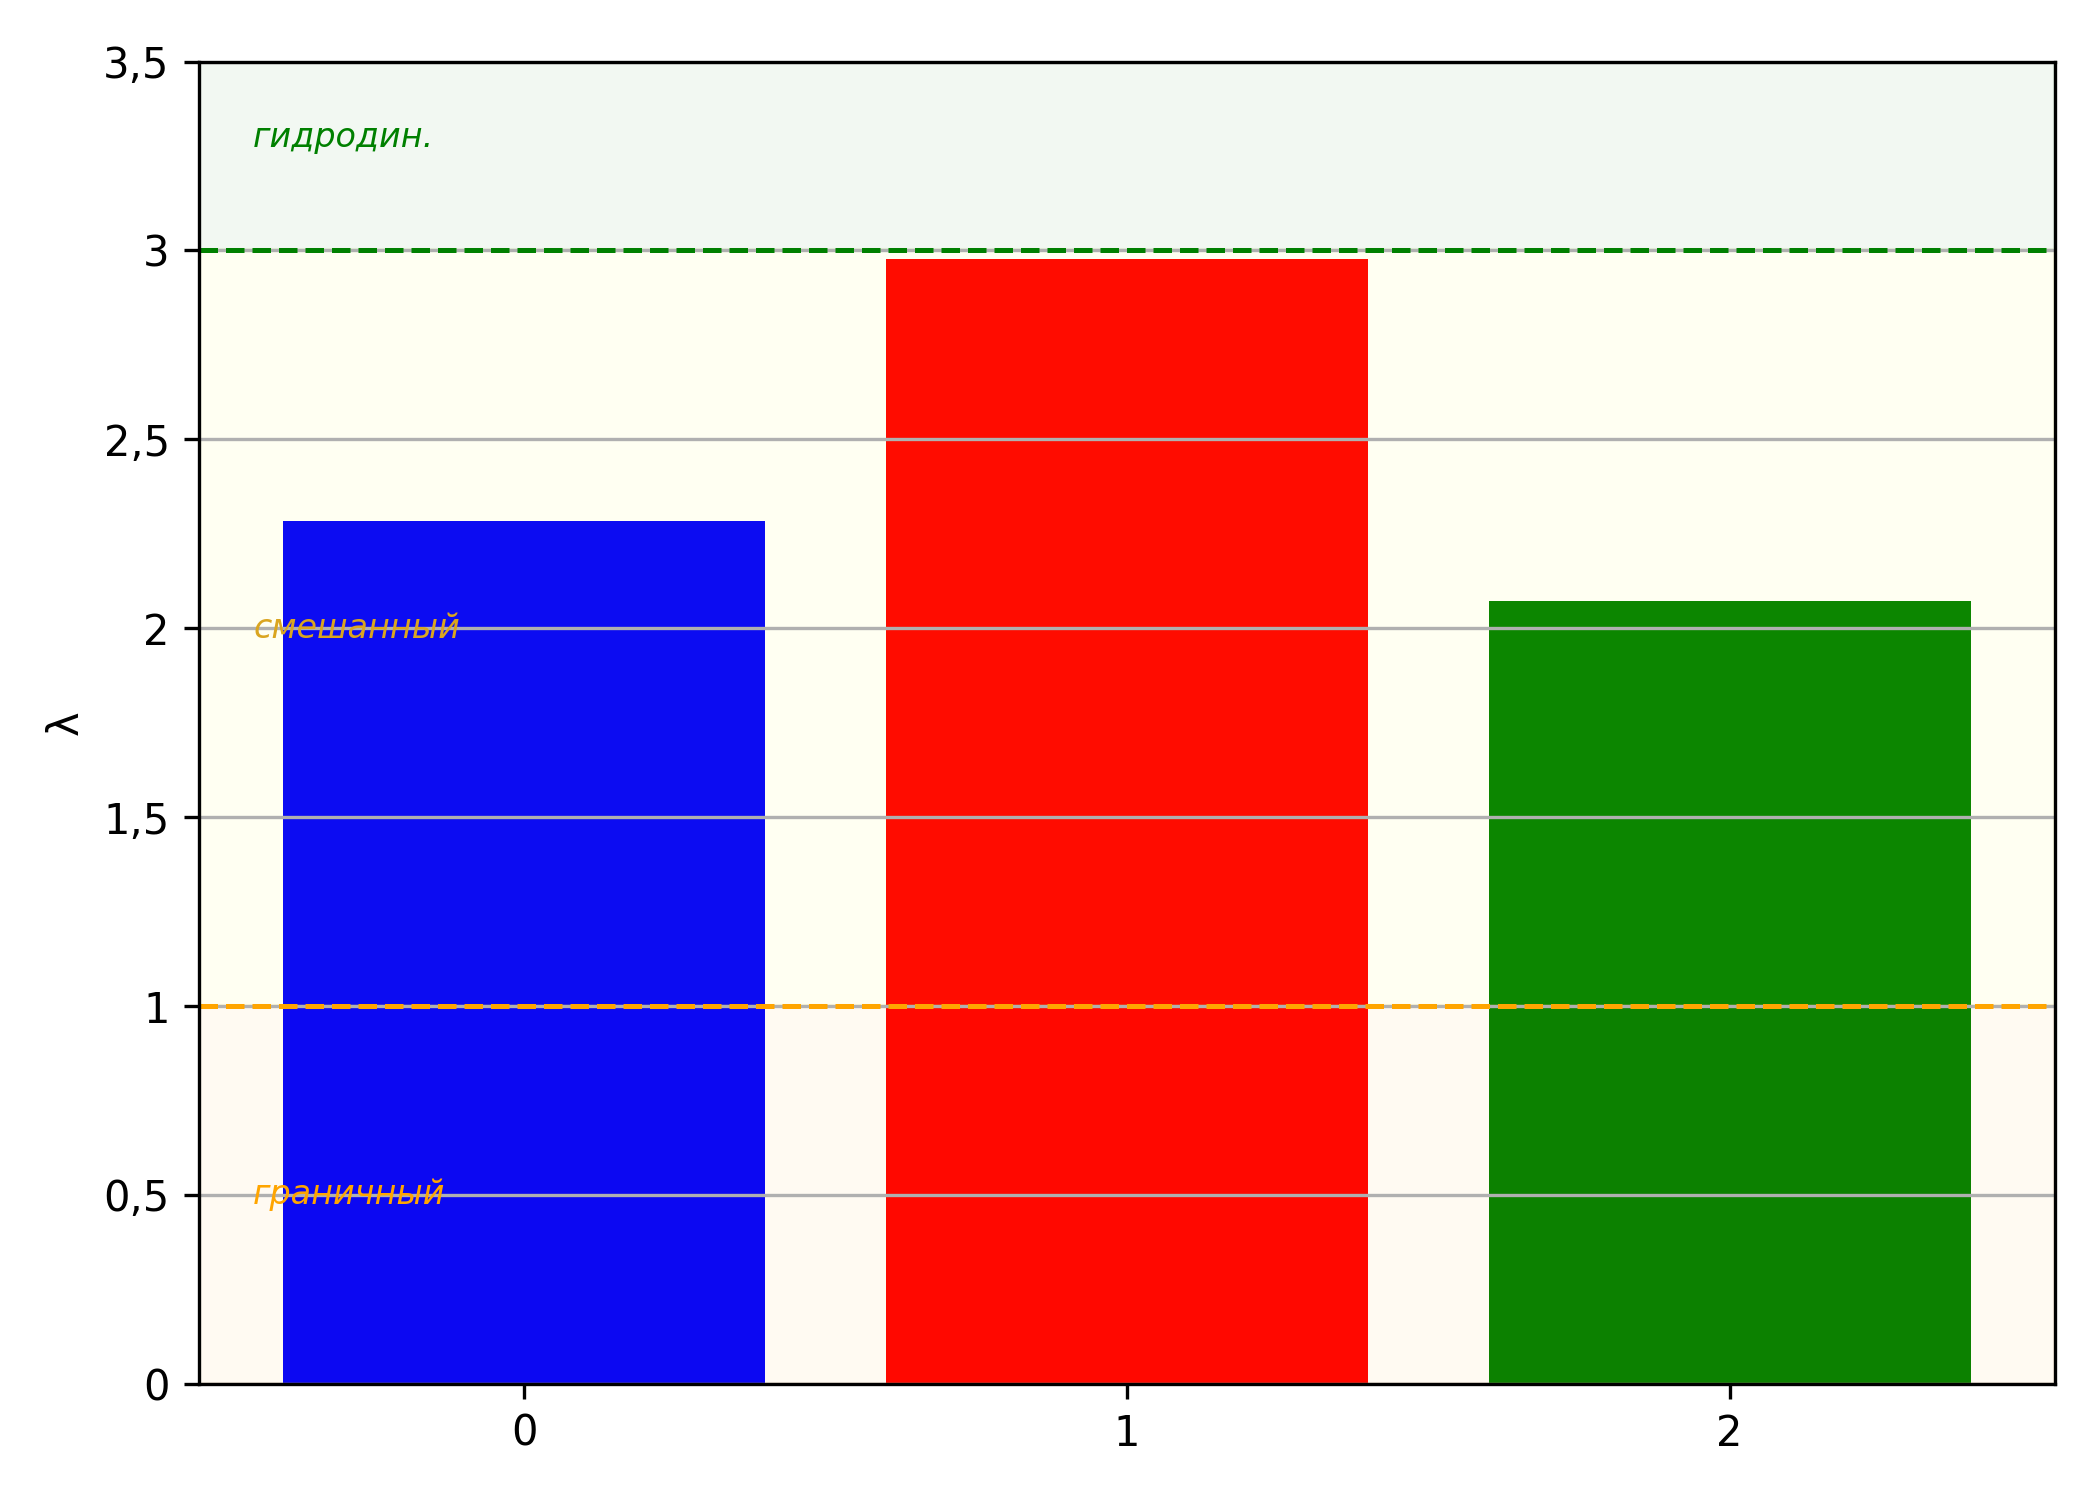
\includegraphics[width=\textwidth,height=0.9\textheight,keepaspectratio]{figures/ch06/fig_6_3.png}
\caption{Параметр плёнки $\lambda$ в рабочей точке ($F_{\mathrm{ext}} = 6\,000$~Н)
  для конфигураций T1, T2, T3. Пунктирные линии~-- границы режимов смазки:
  $\lambda = 1$ и $\lambda = 3$.}
\label{fig:bit_lambda_comparison}
\end{figure}

\FloatBarrier


\textit{Зависимости характеристик от нагрузки.}
Для оценки поведения подшипника при различных условиях нагружения
выполнен параметрический расчёт при~$F_{\mathrm{ext}}$ от
${\sim}\,2100$ до ${\sim}\,6800$~Н. Диапазон ограничен
грузоподъёмностью конфигураций при $\varepsilon = 0{,}97$.

С ростом нагрузки эксцентриситет монотонно возрастает
(рисунок~\ref{fig:bit_sweep_B_epsilon}). При одинаковой
нагрузке конфигурация~T2 имеет наименьший эксцентриситет,
T3~-- наибольший. Конфигурация~T3 достигает расчётного предела
при $F \approx 6200$~Н и теряет рабочую точку раньше, чем T1 и~T2.

\begin{figure}[!ht]
\centering
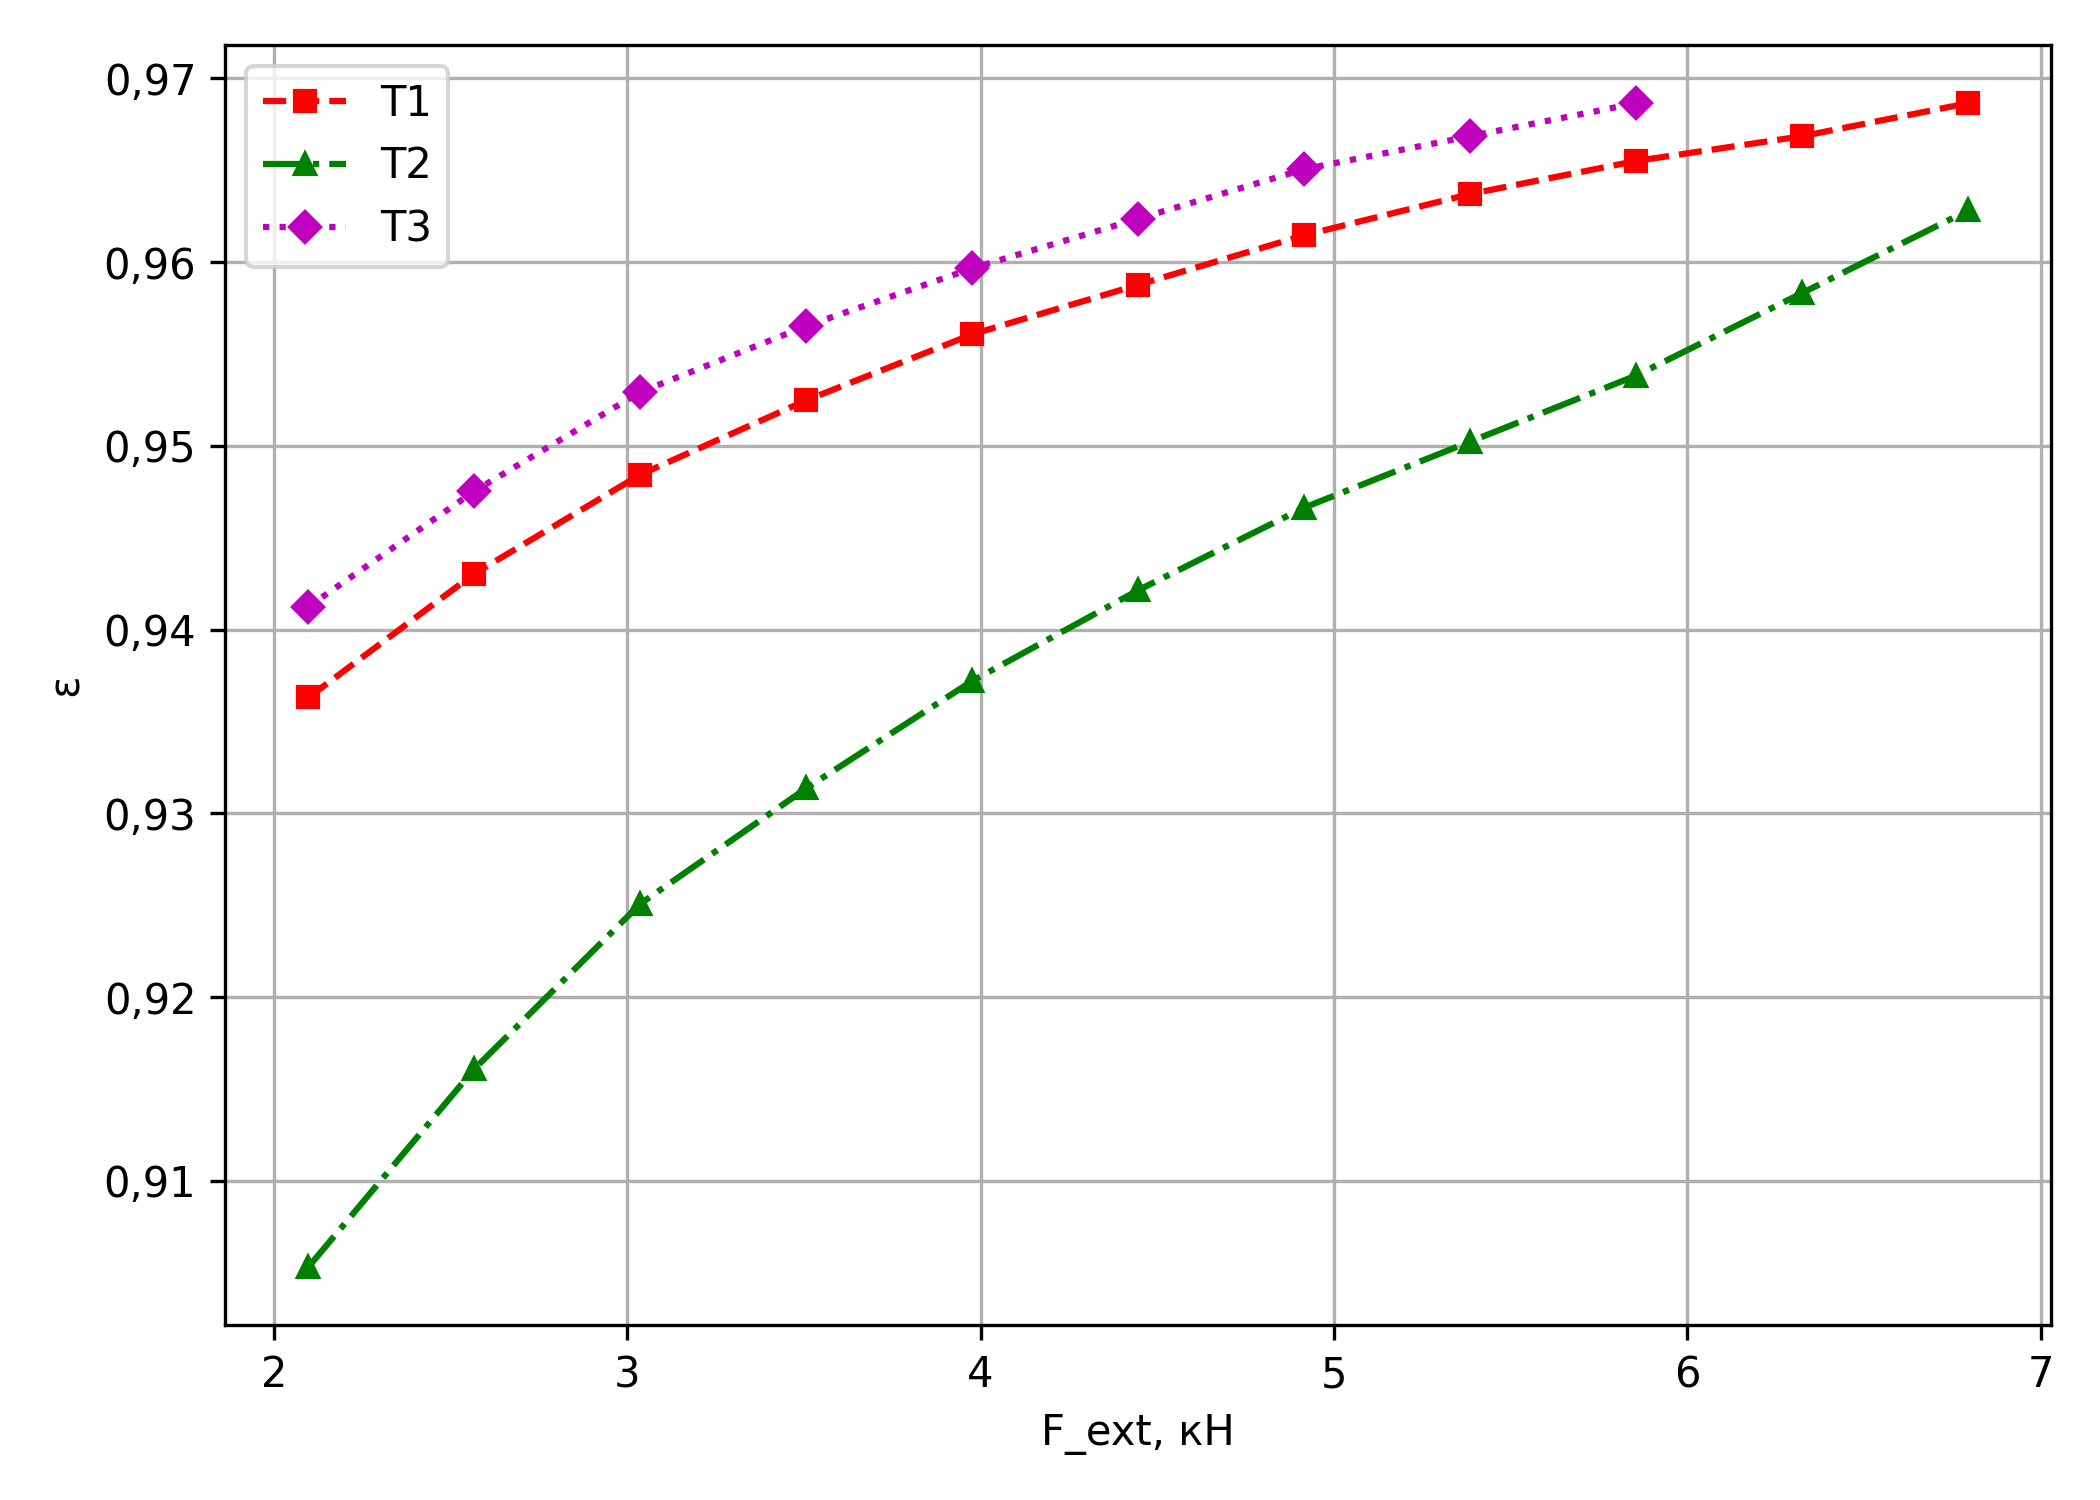
\includegraphics[width=\textwidth,height=0.9\textheight,keepaspectratio]{figures/ch06/fig_6_4.png}
\caption{Зависимость эксцентриситета $\varepsilon$ от нагрузки $F_{\mathrm{ext}}$
  для конфигураций T1, T2, T3 в рабочей зоне текстурированных вариантов.}
\label{fig:bit_sweep_B_epsilon}
\end{figure}

\FloatBarrier

Параметр плёнки~$\lambda$ убывает с ростом нагрузки
(рисунок~\ref{fig:bit_sweep_B_lambda}). При
$F \approx 6\,000$~Н конфигурация~T2 находится вблизи границы
смешанного и гидродинамического режимов ($\lambda \approx 3$);
конфигурации~T1 и~T3 остаются в смешанном режиме ($\lambda < 2{,}5$).

\begin{figure}[!ht]
\centering
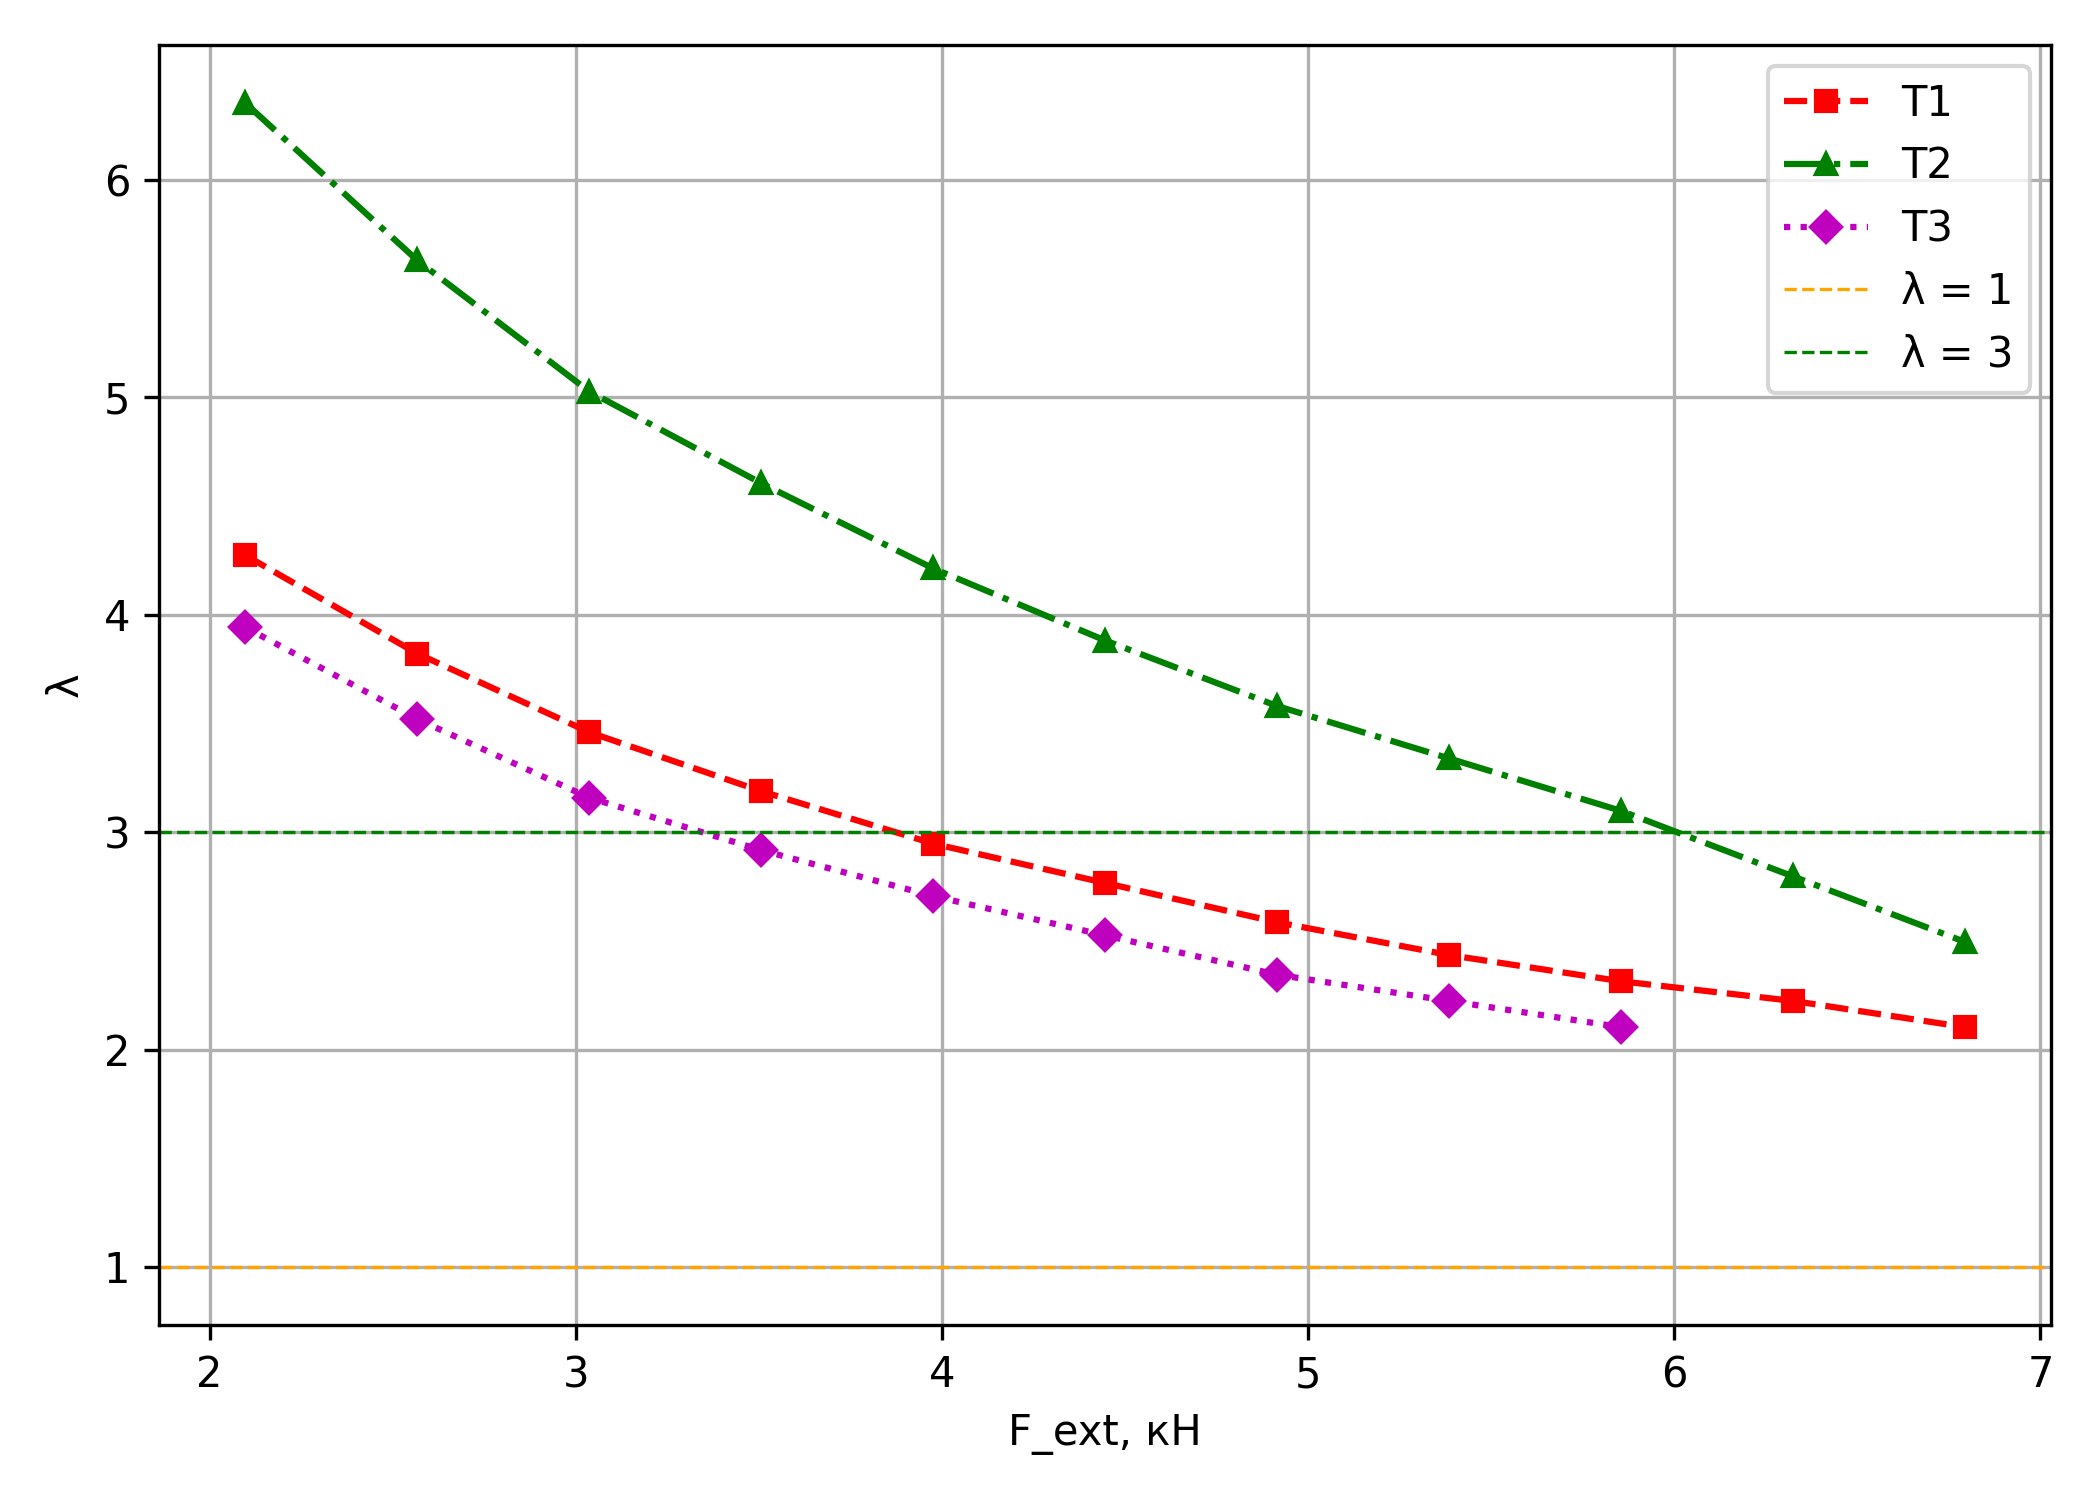
\includegraphics[width=\textwidth,height=0.9\textheight,keepaspectratio]{figures/ch06/fig_6_5.png}
\caption{Зависимость параметра плёнки $\lambda$ от нагрузки $F_{\mathrm{ext}}$.
  Пунктирные линии~-- границы режимов смазки $\lambda = 1$ и $\lambda = 3$.}
\label{fig:bit_sweep_B_lambda}
\end{figure}

\FloatBarrier

Минимальная толщина плёнки~$h_{\min}$ убывает с ростом нагрузки
(рисунок~\ref{fig:bit_sweep_B_hmin}). При $F = 6\,000$~Н:
$h_{\min} = 2{,}66$~мкм (T2), $2{,}04$~мкм (T1), $1{,}85$~мкм (T3),
что сопоставимо с суммарной шероховатостью
$\sigma_{\mathrm{eq}} = 0{,}89$~мкм.

\textit{Коэффициенты улучшения на общей достижимой нагрузке.}
При $F_{\mathrm{ext}} = 6\,000$~Н гладкий подшипник не имеет
рабочей точки, что исключает прямое нормирование характеристик
текстурированных вариантов на значения гладкого при рабочей нагрузке.
Нормированные показатели определяются при общей достижимой нагрузке:

\begin{figure}[!ht]
\centering
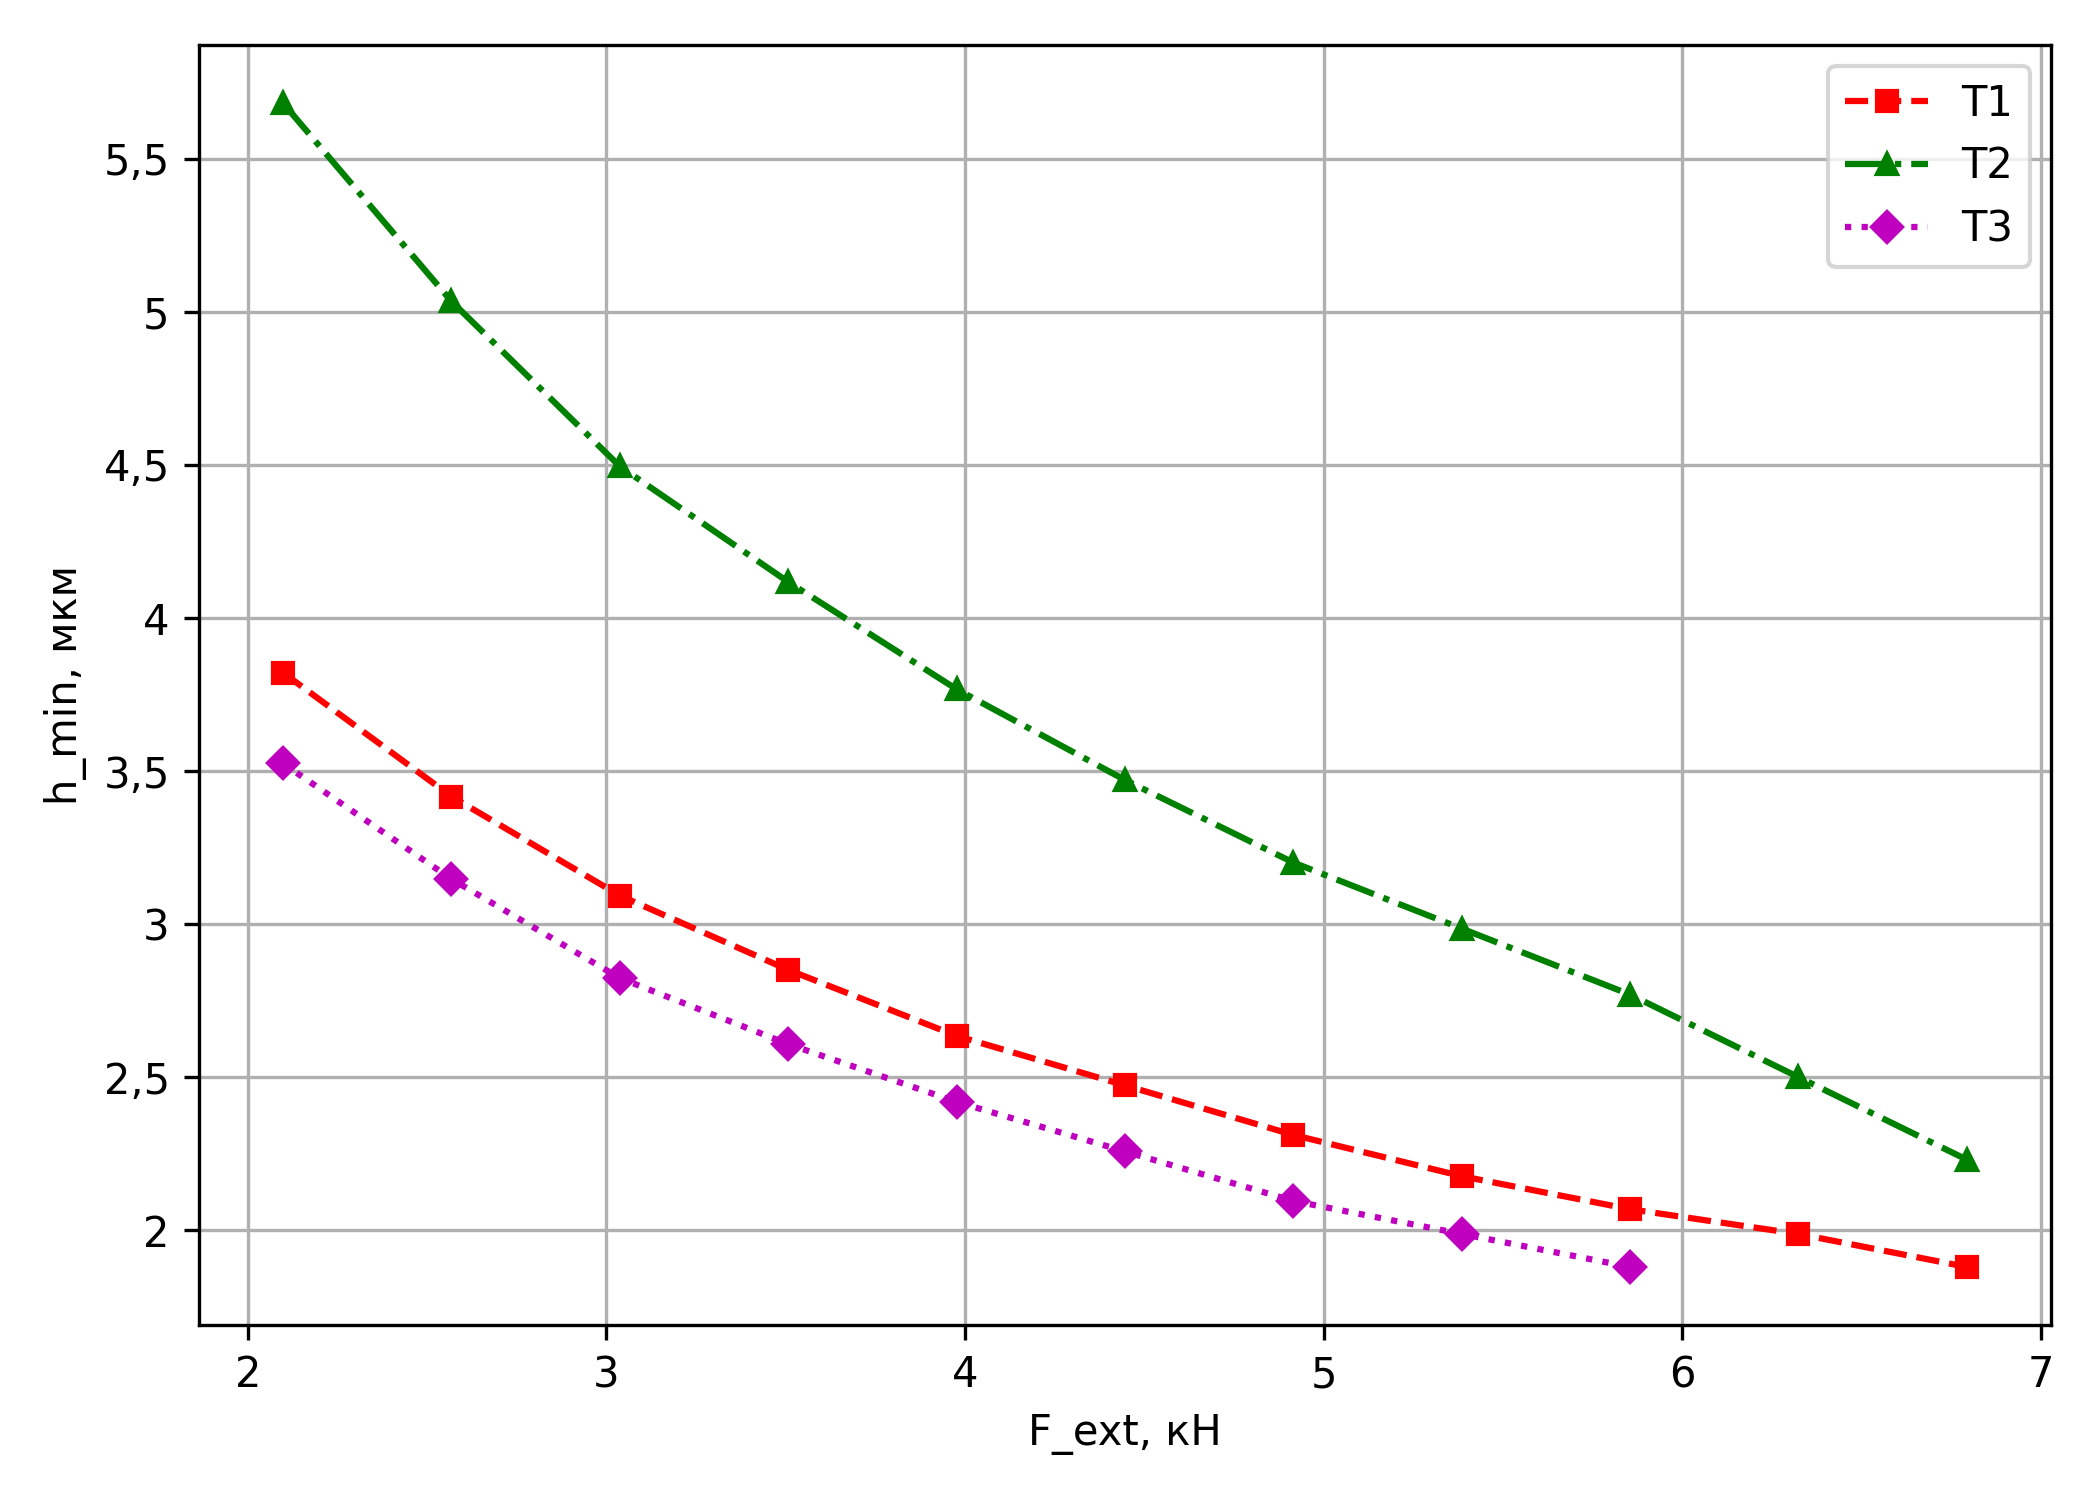
\includegraphics[width=\textwidth,height=0.9\textheight,keepaspectratio]{figures/ch06/fig_6_6.png}
\caption{Зависимость минимальной толщины плёнки $h_{\min}$ от нагрузки
  $F_{\mathrm{ext}}$ для конфигураций T1, T2, T3.}
\label{fig:bit_sweep_B_hmin}
\end{figure}
\begin{equation}
  F_* = 0{,}85 \cdot F_0
    (\varepsilon = 0{,}97) = 1\,621\;\text{Н},
  \label{eq:bit_Fcommon}
\end{equation}
при которой рабочая точка существует у всех вариантов, включая
гладкий.

Нормированные показатели эффективности определяются следующим
образом:
\begin{equation}
\begin{split}
  &G_{h}^{(i)} = \frac{h_{\min}^{(i)}}{h_{\min}^{(0)}},
  \quad
  G_{\lambda}^{(i)} = \frac{\lambda^{(i)}}{\lambda^{(0)}}, \\
  &G_{PV}^{(i)} = \frac{PV^{(0)}}{PV^{(i)}},
  \quad
  G_{w}^{(i)} = \frac{I_w^{(0)}}{I_w^{(i)}}.
\end{split}
  \label{eq:bit_gain_factors}
\end{equation}
где верхний индекс~$(0)$~-- гладкий вариант,
$(i)$~-- текстурированные конфигурации T1, T2, T3.
Значение~$G > 1$ желательно для всех четырёх показателей.

Результаты расчёта нормированных показателей при
$F_* = 1\,621$~Н сведены в
таблицу~\ref{tab:bit_gains}.

\begin{table}[!ht]
\centering
\caption{Нормированные показатели эффективности при
  $F_* = 1\,621$~Н}
\label{tab:bit_gains}
\begin{tabularx}{\textwidth}{|X|c|c|c|c|}
\hline
\multicolumn{1}{|c|}{\textbf{Конфигурация}}
  & $\boldsymbol{G_h}$
  & $\boldsymbol{G_{\lambda}}$
  & $\boldsymbol{G_{PV}}$
  & $\boldsymbol{G_w}$ \\
\hline
T1 & 2{,}119 & 2{,}119 & 1{,}009 & 2{,}137 \\
\hline
T2 & 3{,}147 & 3{,}147 & 1{,}002 & 3{,}153 \\
\hline
T3 & 1{,}964 & 1{,}964 & 0{,}996 & 1{,}956 \\
\hline
\end{tabularx}
\end{table}

\FloatBarrier

Конфигурация~T2 обеспечивает $G_h = 3{,}147$
и $G_{\lambda} = 3{,}147$~-- утроение минимального зазора
и параметра плёнки по сравнению с гладким подшипником.
Показатель~$G_{PV}$ у всех конфигураций близок к единице:
при фиксированной нагрузке номинальное давление~$p_0$
практически не изменяется, и основной эффект текстурирования
реализуется через снижение эксцентриситета и рост зазора,
а не через изменение~$PV$. У конфигурации~T3
$G_{PV} = 0{,}996 < 1$~-- незначительный рост~$PV$, согласующийся
с меньшей несущей способностью этой конфигурации.

Нормированные показатели наглядно сопоставлены на
рисунке~\ref{fig:bit_gains_common}.

\begin{figure}[!ht]
\centering
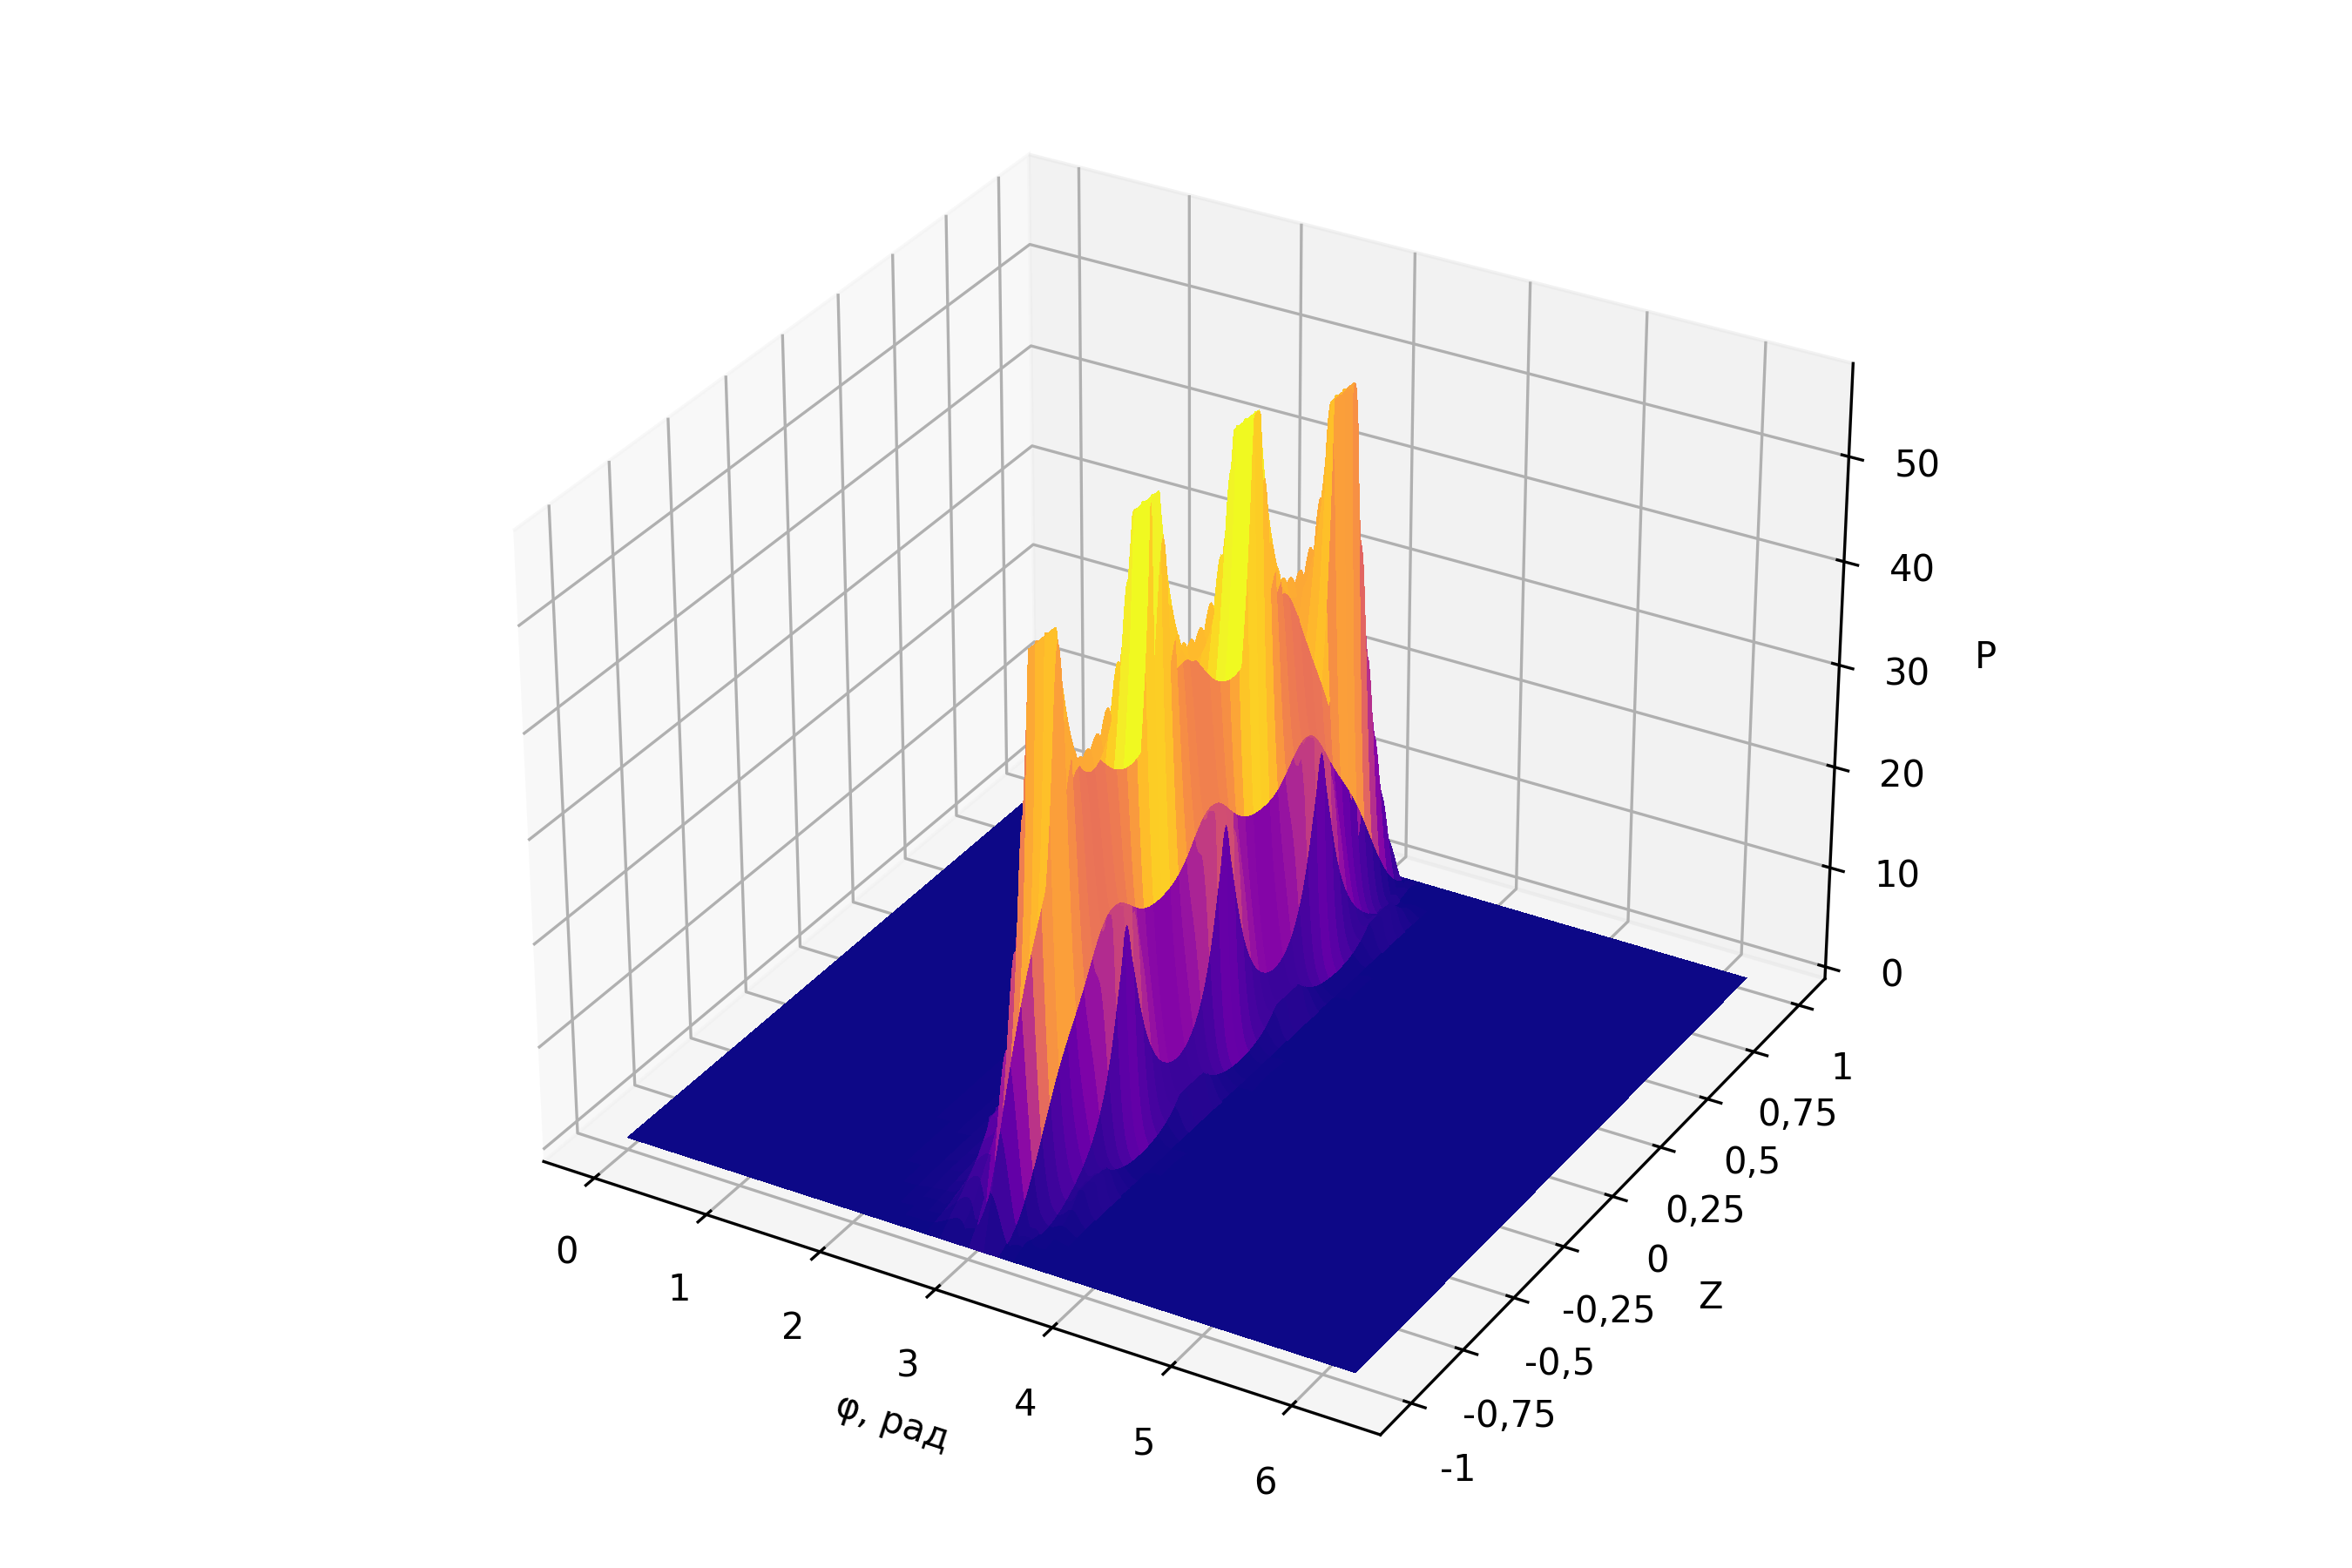
\includegraphics[width=\textwidth,height=0.9\textheight,keepaspectratio]{figures/ch06/fig_6_7.png}
\caption{Нормированные показатели эффективности $G_h$, $G_{\lambda}$,
  $G_{PV}$, $G_w$ для конфигураций T1, T2, T3
  при $F_* = 1\,621$~Н.
  Пунктирная горизонталь $G = 1$~-- уровень гладкого подшипника.}
\label{fig:bit_gains_common}
\end{figure}

\FloatBarrier


\textit{Поле давления лучшей конфигурации.}
Для конфигурации~T2, продемонстрировавшей наилучшие характеристики,
представлено трёхмерное поле безразмерного давления~$P(\theta, Z)$
в рабочей точке ($\varepsilon = 0{,}956$). Зона максимального
давления располагается вблизи $\theta \approx \pi$. Лунки
конфигурации~T2 формируют выраженную <<рябь>> на поверхности
давления, свидетельствующую о локальном перераспределении потоков
в каждом элементе микрорельефа
(рисунок~\ref{fig:bit_P3D_T2}).

\begin{figure}[!ht]
\centering
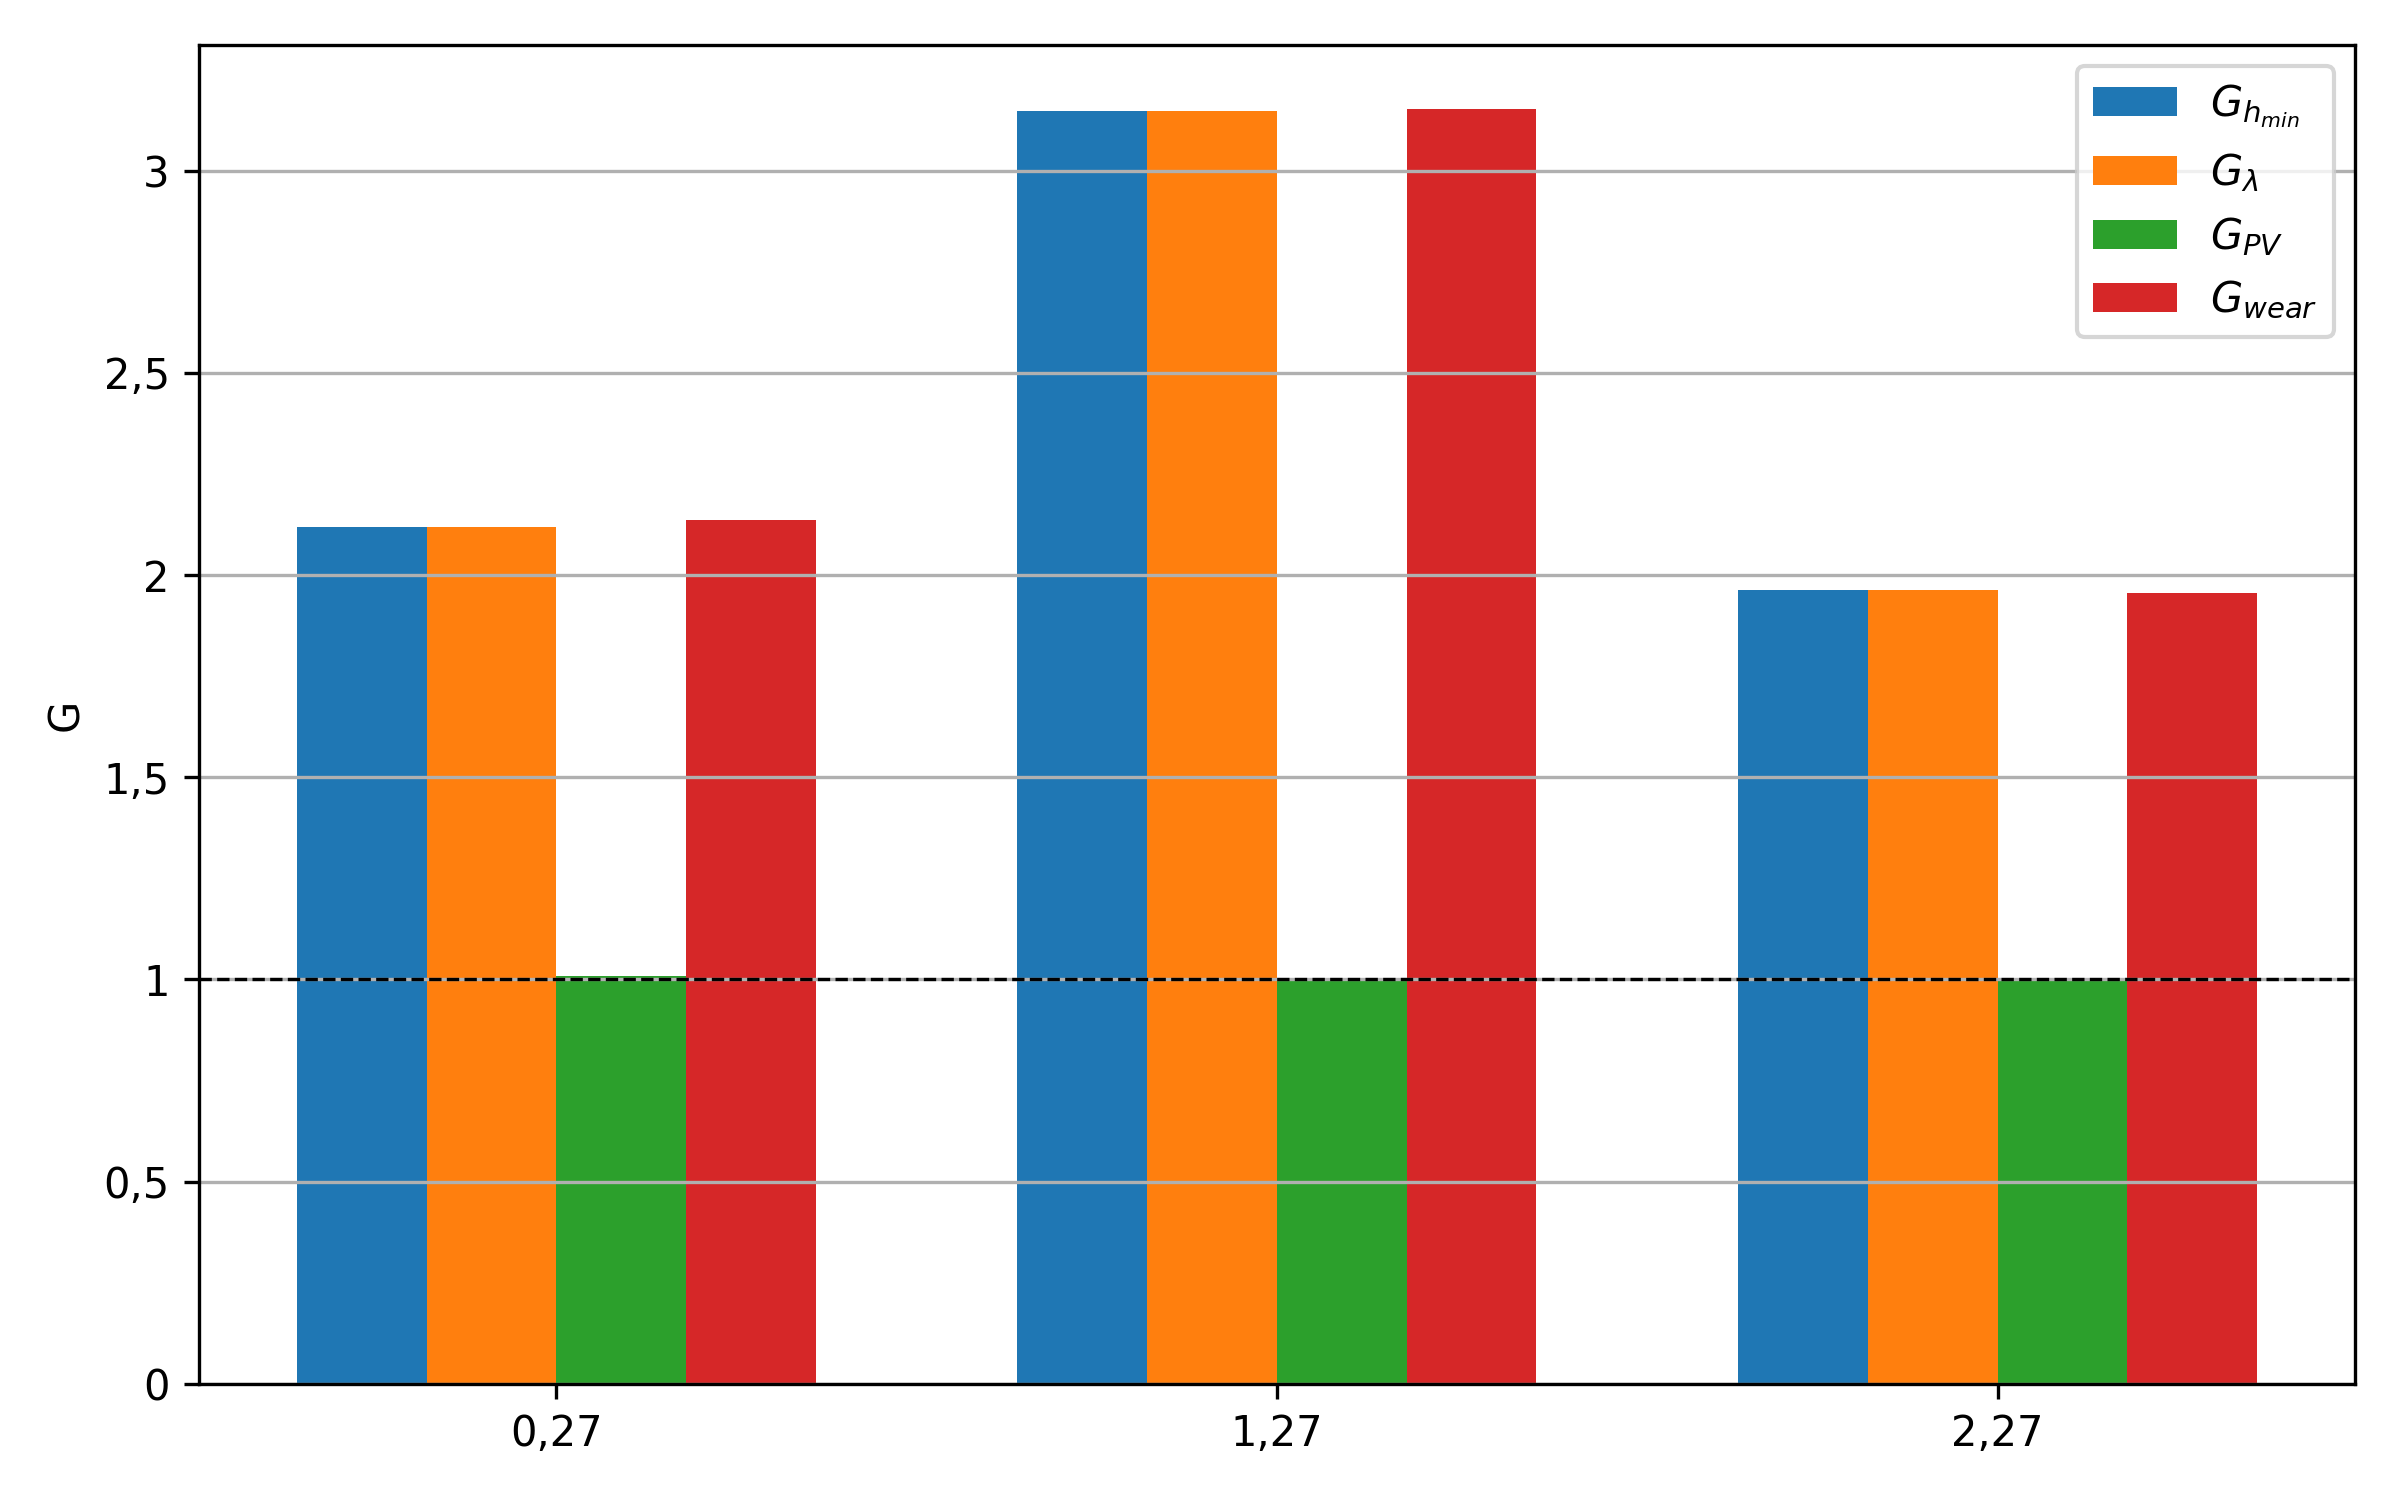
\includegraphics[width=\textwidth,height=0.9\textheight,keepaspectratio]{figures/ch06/fig_6_8.png}
\caption{Поле безразмерного давления $P(\theta, Z)$
  для конфигурации~T2 ($H_p = 0{,}40$, зона $90^{\circ}$--$270^{\circ}$)
  в рабочей точке $\varepsilon = 0{,}956$.}
\label{fig:bit_P3D_T2}
\end{figure}


\FloatBarrier
\section*{Выводы по главе~6}
\phantomsection\addcontentsline{toc}{section}{Выводы по главе~6}

Проведён анализ радиального подшипника скольжения опоры шарошки
трёхшарошечного долота в изотермическом приближении с учётом
кавитации по условию Рейнольдса ($P \geq 0$). Установлено, что
гладкий подшипник при рабочей нагрузке
$F_{\mathrm{ext}} = 6\,000$~Н не имеет равновесной рабочей точки
в чисто гидродинамической постановке:
$F(\varepsilon = 0{,}97) = 1907$~Н.

Текстурирование поверхности цапфы эллипсоидальными лунками
в шахматной раскладке существенно повышает гидродинамическую
несущую способность: $F(\varepsilon = 0{,}97)$ достигает
$7549$~Н (конфигурация~T2), что в~$3{,}96$ раза превышает
значение гладкого варианта. Рабочая точка при
$F_{\mathrm{ext}} = 6\,000$~Н найдена для всех конфигураций
T1--T3.

В рабочих точках все конфигурации функционируют в смешанном режиме
смазки ($\lambda \approx 2{,}1$--$3{,}0$). Конфигурация~T2
($H_p = 0{,}40$, зона $90^{\circ}$--$270^{\circ}$) демонстрирует
наилучшие показатели: $\varepsilon = 0{,}956$,
$h_{\min} = 2{,}66$~мкм, $\lambda = 2{,}98$~-- значение,
наиболее близкое к границе гидродинамического режима.

На общей достижимой нагрузке $F_* = 1\,621$~Н
конфигурация~T2 обеспечивает трёхкратное увеличение минимального
зазора ($G_h = 3{,}15$) и параметра плёнки
($G_{\lambda} = 3{,}15$). Показатели~$G_{PV}$ близки к единице
(фиксированная нагрузка); основной эффект текстурирования
реализуется через рост минимального зазора и улучшение условий
смазки.

Анализ упорного подшипника скольжения с детерминированными
микроструктурами выполнен в главе~7.
